% =====================================================================
%  第 2 章 路径积分形式 —— ch02a（章首 + §2.1–§2.5 前半）
%  页段：PDF 81–108（原书 p.80–107）
% =====================================================================

\chapter{路径积分形式}

% [原文 p.80]
本章讲解量子力学的路径积分方法，它以概率式的路径刻画粒子的量子动力学。这个形式提供了计算跃迁振幅、理解量子现象的有力工具，在现代量子场论中已被广泛推广与发展。本章的讲述重在直觉与例子，用它们阐明基本想法。

\section{路径积分引论}

\subsection{量子演化与费曼核}

我们此前用波函数 $\psi$（希尔伯特空间中的向量）讨论量子力学的状态空间，用薛定谔方程给出量子时间演化的规律
\[
\ii\hbar\frac{\pa}{\pa t}\psi=\hat H\psi.
\]
这里 $\hat H$ 是哈密顿算子（也称薛定谔算子），它是把经典哈密顿函数 $\mathcal H$ 量子化的微分算子。

本章只考虑不依赖时间的 $\hat H$。把 $\hat H$ 看作状态希尔伯特空间上的自伴算子，则薛定谔方程给出的态的时间演化为
\[
\ket{\psi(t'')}=\ee^{-\ii\hat H(t''-t')/\hbar}\ket{\psi(t')},
\qquad t'<t''.
\]
于是，量子力学中的时间演化完全编码在希尔伯特空间上单参数族的酉算子 $\ee^{-\ii\hat Ht/\hbar}$ 之中。

我们将会看到，算子 $\ee^{-\ii\hat Ht/\hbar}$ 可由一个积分核表示。这意味着波函数 $\psi(\mathbf{x},t)$ 的演化可写成积分关系
\[
\psi(\mathbf{x}'',t'')
=\int\rd\mathbf{x}'\,K(\mathbf{x}'',t'';\mathbf{x}',t')\psi(\mathbf{x}',t').
\]
这个积分核 $K$ 在量子力学的另一种表述中唱主角：\emph{路径积分}（path integral）方法。

经典力学中，最小作用量原理起主导作用。经典系统通常用作用量泛函描述
\[
S[\mathbf{x}(t)]=\int\rd t\,\mathcal L(\mathbf{x}(t),\dot{\mathbf{x}}(t)),
\]

% [原文 p.81]
其中 $\mathcal L$ 称为\emph{拉格朗日量}（Lagrangian）。经典粒子的轨迹是作用量 $S$ 的驻点，可用欧拉–拉格朗日方程描述
\[
\frac{\pa\mathcal L}{\pa x_i}
-\frac{\rd}{\rd t}\left(\frac{\pa\mathcal L}{\pa\dot x_i}\right)=0.
\]
经典力学的这一拉格朗日表述与哈密顿表述通过勒让德变换相联系
\[
\mathcal H(\mathbf{x},\mathbf{p})=\mathbf{p}\cdot\dot{\mathbf{x}}-\mathcal L(\mathbf{x},\dot{\mathbf{x}}).
\]
这里 $p_i=\dfrac{\pa\mathcal L}{\pa\dot x_i}$ 是从 $\dot{\mathbf{x}}$ 出发的勒让德变换，称为 $x_i$ 的\emph{共轭动量}（conjugate momentum）。

引人注目的是，对这个积分核 $K$ 的研究直接通到拉格朗日表述！这最早是狄拉克在研究量子力学中共轭变量的正则变换时注意到的。这一观点在费曼之前并未真正用上，是费曼给出了「量子力学的路径积分方法」的完整故事。在这个故事里，积分核 $K$ 被解释为对路径空间的「积分」
\[
K(\mathbf{x}'',t'';\mathbf{x}',t')
=\int_{\mathbf{x}(t')=x'}^{\mathbf{x}(t'')=x''}[D\mathbf{x}(t)]\,
\ee^{\frac{\ii}{\hbar}S[\mathbf{x}(t)]}.
\]

\begin{center}
  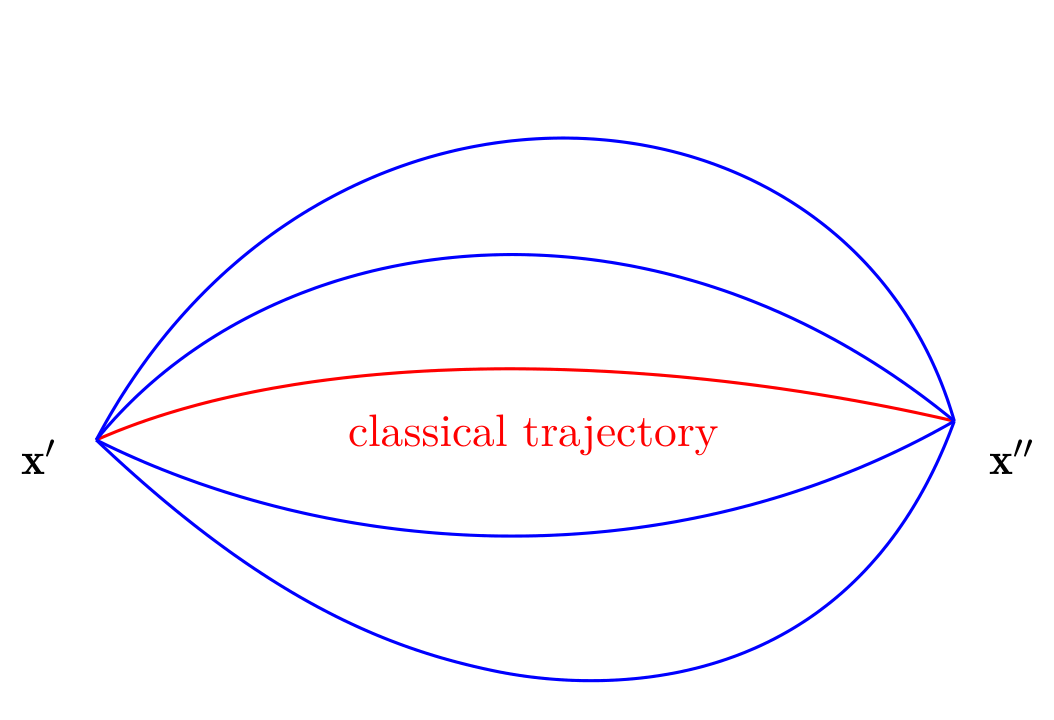
\includegraphics[width=0.62\textwidth]{figures/fig_p82_a.png}
\end{center}
% [图：原书 p.81，原图无题注]
\fignote{图内文字：classical trajectory（译：经典轨迹）}

这里 $[D\mathbf{x}(t)]$ 应当是对路径空间的某种测度
\[
\mathbf{x}:[t',t'']\longrightarrow\text{空间},
\]
端点条件为 $\mathbf{x}(t')=\mathbf{x}'$、$\mathbf{x}(t'')=\mathbf{x}''$。

一个关键特征是：所有路径都通过作用量泛函 $S$ 对积分核 $K$ 作出贡献。这个表达式给出了经典力学与量子力学之间的直接联系。在 $\hbar\to 0$ 的经典极限下，驻定相位方法提示，上述路径积分的主要贡献来自驻定路径，而它们恰是经典轨迹！这一干净而直观的解释已被推广、应用到许多量子物理问题，如今已是教科书的标配。

遗憾的是，路径空间极大，且是无穷维的。在我们关心的许多量子力学情形中，这可以与马尔可夫演化、布朗

% [原文 p.82]
运动联系起来，于是维纳测度可用。至于量子场论中的一般路径积分，相应测度的严格数学构造至今未知。这已成为现代量子理论的主要基础性难题之一。

尽管如此，路径积分方法为许多量子问题提供了深刻洞见。即使没有一般的严格测度可用，我们在物理中仍能做大量具体计算。事实上，费曼发展路径积分形式的一大动机，就是用它在量子电动力学中做研究。路径积分计算能力的一个原因就在形式本身。对通常的有限维积分
\[
\int f
\]
我们几乎从不按黎曼积分或勒贝格积分的定义去算它，而是用对称性和由积分的某些形式、自然性质导出的微分方程去算。物理中操作路径积分的处境一般也是如此。只要承认若干从普通积分借来的自然初等性质，我们就能做许多具体计算。

上面这套路径积分的故事也称\emph{费曼路径积分}（Feynman path integral）。积分核 $K$ 在文献中通常称为\emph{费曼核}（Feynman kernel）。

\subsection{位置与动量表示}

我们将主要关注希尔伯特空间
\[
L^2(\R^n).
\]
态 $\psi(\mathbf{x})\in L^2(\R^n)$ 是平方可积的可测函数
\[
\int\rd^n\mathbf{x}\,|\psi(\mathbf{x})|^2<\infty.
\]
内积为
\[
\braket{\psi_1}{\psi_2}=\int\rd^n\mathbf{x}\,
\overline{\psi_1(\mathbf{x})}\,\psi_2(\mathbf{x}).
\]
引入位置算子 $\hat{\mathbf{x}}$ 的本征向量 $\ket{\mathbf{x}'}$ 会带来方便，其定义是
\[
\hat x_i\ket{\mathbf{x}'}=x_i'\ket{\mathbf{x}'}.
\]
严格说来，$\ket{\mathbf{x}'}$ 并不落在希尔伯特空间里，它对应自伴算子 $\hat{\mathbf{x}}$ 的连续谱。$\ket{\mathbf{x}'}$ 的「波函数」是 $\delta$ 函数
\[
\ket{\mathbf{x}'}\ \sim\ \delta(\mathbf{x}-\mathbf{x}'),
\]
它不可归一。这个态位于缓增广义函数空间中。尽管如此，我们仍可形式地使用这类态，以简化许多表述。例如，可以把位置算子的全部本征向量当作一组「基」，其内积归一为
\[
\braket{\mathbf{x}''}{\mathbf{x}'}=\delta(\mathbf{x}''-\mathbf{x}').
\]

% [原文 p.83]
任一态 $\ket{\psi}$ 可按这组基展开为
\[
\ket{\psi}=\int\rd^n\mathbf{x}\,\psi(\mathbf{x})\ket{\mathbf{x}}.
\]
于是波函数可解释为态在这样一组位置本征向量基下的系数。等价地，可以写
\[
\psi(\mathbf{x})=\braket{\mathbf{x}}{\psi}.
\]
这可由下式验证：
\[
\braket{\mathbf{x}}{\psi}
=\bra{\mathbf{x}}\int\rd^n\mathbf{x}'\,\psi(\mathbf{x}')\ket{\mathbf{x}'}
=\int\rd^n\mathbf{x}'\,\psi(\mathbf{x}')\braket{\mathbf{x}}{\mathbf{x}'}
=\int\rd^n\mathbf{x}'\,\psi(\mathbf{x}')\delta(\mathbf{x}-\mathbf{x}')
=\psi(\mathbf{x}).
\]
我们也可把公式
\[
\ket{\psi}=\int\rd^n\mathbf{x}\,\braket{\mathbf{x}}{\psi}\ket{\mathbf{x}}
=\int\rd^n\mathbf{x}\,\ket{\mathbf{x}}\braket{\mathbf{x}}{\psi}
\]
改写成完备性关系
\[
\int\rd^n\mathbf{x}\,\ket{\mathbf{x}}\bra{\mathbf{x}}=1,
\]
其中 $1$ 表示恒等算子。

类似地，可引入动量算子 $\hat{\mathbf{p}}$ 的本征向量 $\ket{\mathbf{p}'}$，定义为
\[
\hat p_i\ket{\mathbf{p}'}=p_i'\ket{\mathbf{p}'}.
\]
按我们的约定，其归一为
\[
\braket{\mathbf{p}''}{\mathbf{p}'}=(2\pi\hbar)^n\delta(\mathbf{p}''-\mathbf{p}').
\]
于是完备性关系成为
\[
\frac{1}{(2\pi\hbar)^n}\int\rd^n\mathbf{p}\,\ket{\mathbf{p}}\bra{\mathbf{p}}=1.
\]
位置本征向量与动量本征向量由傅里叶变换相联系
\[
\ket{\mathbf{p}}=\int\rd^n\mathbf{x}\,\ee^{\ii\mathbf{x}\cdot\mathbf{p}/\hbar}\ket{\mathbf{x}},
\]
等价地
\[
\braket{\mathbf{x}}{\mathbf{p}}=\ee^{\ii\mathbf{x}\cdot\mathbf{p}/\hbar}.
\]
取复共轭得
\[
\braket{\mathbf{p}}{\mathbf{x}}=\ee^{-\ii\mathbf{x}\cdot\mathbf{p}/\hbar}.
\]
态 $\ket{\psi}$ 既可按位置本征向量展开，得到
\[
\psi(\mathbf{x})=\braket{\mathbf{x}}{\psi},
\]
也可按动量本征向量展开，得到
\[
\hat\psi(\mathbf{p})=\braket{\mathbf{p}}{\psi}.
\]

% [原文 p.84]
两者由下式相联系：
\[
\psi(\mathbf{x})=\braket{\mathbf{x}}{\psi}
=\bra{\mathbf{x}}\frac{1}{(2\pi\hbar)^n}\int\rd^n\mathbf{p}\,
\ket{\mathbf{p}}\braket{\mathbf{p}}{\psi}
=\frac{1}{(2\pi\hbar)^n}\int\rd^n\mathbf{p}\,
\ee^{\ii\mathbf{x}\cdot\mathbf{p}/\hbar}\,\hat\psi(\mathbf{p}),
\]
\[
\hat\psi(\mathbf{p})=\braket{\mathbf{p}}{\psi}
=\bra{\mathbf{p}}\int\rd^n\mathbf{x}\,\ket{\mathbf{x}}\braket{\mathbf{x}}{\psi}
=\int\rd^n\mathbf{x}\,\ee^{-\ii\mathbf{x}\cdot\mathbf{p}/\hbar}\,\psi(\mathbf{x}),
\]
而这恰是傅里叶变换公式。

\takeaway{薛定谔方程的时间演化由单参数族酉算子 $\ee^{-\ii\hat Ht/\hbar}$ 给出，它的积分核 $K$ 称为费曼核。路径积分把 $K$ 解释为对连接两端点的所有路径按 $\ee^{\ii S/\hbar}$ 加权求和；$\hbar\to0$ 时，驻定相位使主要贡献来自作用量的驻点，即经典轨迹。}

我们可以用上面的表示来写出积分核 $K$。设 $\ket{\psi}$ 是 $t=0$ 时的初始态。记 $\ket{\psi,t}$ 为 $t$ 时刻的态，从而 $\ket{\psi}=\ket{\psi,0}$。于是
\[
\ket{\psi,t}=\ee^{-\ii\hat Ht/\hbar}\ket{\psi}.
\]
相应的波函数为
\[
\psi(\mathbf{x},t)=\braket{\mathbf{x}}{\psi,t}
=\bra{\mathbf{x}}\ee^{-\ii\hat Ht/\hbar}\ket{\psi}.
\]
若在两个不同时刻 $t'$ 与 $t''$ 作比较，
\[
\begin{aligned}
\psi(\mathbf{x}'',t'')
&=\bra{\mathbf{x}''}\ee^{-\ii\hat Ht''/\hbar}\ket{\psi}
=\bra{\mathbf{x}''}\ee^{-\ii\hat H(t''-t')/\hbar}\ee^{-\ii\hat Ht'/\hbar}\ket{\psi}\\
&=\bra{\mathbf{x}''}\ee^{-\ii\hat H(t''-t')/\hbar}
\left(\int\rd^n\mathbf{x}'\,\ket{\mathbf{x}'}\bra{\mathbf{x}'}\right)
\ee^{-\ii\hat Ht'/\hbar}\ket{\psi}\\
&=\int\rd^n\mathbf{x}'\,
\bra{\mathbf{x}''}\ee^{-\ii\hat H(t''-t')/\hbar}\ket{\mathbf{x}'}
\,\psi(\mathbf{x}',t'),
\end{aligned}
\]
我们就得到费曼核 $K$ 的如下表达式
\[
K(\mathbf{x}'',t'';\mathbf{x}',t')
=\bra{\mathbf{x}''}\ee^{-\ii\hat H(t''-t')/\hbar}\ket{\mathbf{x}'}.
\]
总之，可以把 $K(\mathbf{x}'',t'';\mathbf{x}',t')$ 看作演化算子 $\ee^{-\ii\hat H(t''-t')/\hbar}$ 在位置本征向量基下的矩阵元。

\section{时间切片下的路径积分}

\subsection{自由粒子}

我们从自由粒子的例子开始研究费曼核 $K$。哈密顿量为
\[
\hat H_0=\frac{\hat p^2}{2m},\qquad m=\text{质量}.
\]
记自由粒子的费曼核为 $K_0$
\[
K_0(\mathbf{x}'',t'';\mathbf{x}',t')
=\bra{\mathbf{x}''}\ee^{-\ii\hat H_0(t''-t')/\hbar}\ket{\mathbf{x}'}.
\]
为描述这个核，可以先算
\[
\bra{\mathbf{p}}\ee^{-\ii\hat H_0t/\hbar}\ket{\mathbf{x}}
=\bra{\mathbf{p}}\ee^{-\ii\frac{\hat p^2}{2m}t}\ket{\mathbf{x}}
\overset{\text{用 }\bra{\mathbf{p}}\hat{\mathbf{p}}=\mathbf{p}\bra{\mathbf{p}}}{=}
\ee^{-\ii\frac{p^2}{2m}t}\braket{\mathbf{p}}{\mathbf{x}}
=\ee^{-\ii\frac{p^2}{2m}t}\ee^{-\ii\mathbf{x}\cdot\mathbf{p}/\hbar}.
\]

% [原文 p.85]
由此可知
\[
\begin{aligned}
\bra{\mathbf{x}''}\ee^{-\ii\hat H_0(t''-t')/\hbar}\ket{\mathbf{x}'}
&=\frac{1}{(2\pi\hbar)^n}\int\rd^n\mathbf{p}\,
\braket{\mathbf{x}''}{\mathbf{p}}
\bra{\mathbf{p}}\ee^{-\ii\hat H_0(t''-t')/\hbar}\ket{\mathbf{x}'}\\
&=\frac{1}{(2\pi\hbar)^n}\int\rd^n\mathbf{p}\,
\ee^{-\ii\frac{p^2(t''-t')}{2m\hbar}}\,
\ee^{\ii(\mathbf{x}''-\mathbf{x}')\cdot\mathbf{p}/\hbar}.
\end{aligned}
\]
用高斯积分公式
\[
\int\rd u\,\ee^{-au^2+bu}=\sqrt{\frac{\pi}{a}}\,\ee^{\frac{b^2}{4a}},
\]
上述积分为（严格说来需要作解析延拓，见 §2.5.2）
\[
K_0(\mathbf{x}'',t'';\mathbf{x}',t')
=\left(\frac{m}{2\pi\hbar\ii(t''-t')}\right)^{\frac n2}
\ee^{\ii\frac{m(\mathbf{x}''-\mathbf{x}')^2}{2\hbar(t''-t')}}.
\]
这就给出了自由粒子积分核的显式公式。

\begin{remark}{2.2.1}
注意当时间是纯虚的、且
\[
\ii(t''-t')=\tau>0
\]
并且 $m=\dfrac{\hbar}{2}$ 时，核 $K$ 变成
\[
\frac{1}{(4\pi\tau)^{n/2}}\,\ee^{-\frac{(\mathbf{x}''-\mathbf{x}')^2}{4\tau}},
\]
而这恰是 $\R^n$ 上热算子 $\ee^{\tau\nabla^2}$ 的核。这是意料之中的结果，因为此时 $\hat H_0=-\dfrac{\hbar^2}{2m}\nabla^2=-\hbar\nabla^2$，且
\[
\bra{\mathbf{x}''}\ee^{\tau\nabla^2}\ket{\mathbf{x}'}
=\bra{\mathbf{x}''}\ee^{-\hat H_0\tau/\hbar}\ket{\mathbf{x}'}
=\frac{1}{(4\pi\tau)^{n/2}}\,\ee^{-\frac{(\mathbf{x}''-\mathbf{x}')^2}{4\tau}}.
\]
我们将在 §2.2.5 回到虚时间的讨论。
\end{remark}

\subsection{无穷小时间}

接下来考虑一般哈密顿算子
\[
\hat H=\frac{\hat p^2}{2m}+V(\hat{\mathbf{x}})
\]
在无穷小时间 $\delta t$ 内的演化所对应的费曼核
\[
K(\mathbf{x}'',t+\delta t;\mathbf{x}',t)
=\bra{\mathbf{x}''}\ee^{-\ii\hat H\delta t/\hbar}\ket{\mathbf{x}'}.
\]
保留 $\delta t$ 的一阶项，近似有
\[
\ee^{-\ii\hat H\delta t/\hbar}
\simeq\ee^{-\ii\frac{\hat p^2\delta t}{2m\hbar}}\,
\ee^{-\ii\frac{V(\hat{\mathbf{x}})\delta t}{\hbar}}.
\]
利用上面关于自由费曼核的结果，得
\[
\begin{aligned}
K(\mathbf{x}'',t+\delta t;\mathbf{x}',t)
&\simeq\bra{\mathbf{x}''}\ee^{-\ii\frac{\hat p^2\delta t}{2m\hbar}}
\ee^{-\ii\frac{V(\hat{\mathbf{x}})\delta t}{\hbar}}\ket{\mathbf{x}'}\\
&=\bra{\mathbf{x}''}\ee^{-\ii\frac{\hat p^2\delta t}{2m\hbar}}\ket{\mathbf{x}'}\,
\ee^{-\ii\frac{V(\mathbf{x}')\delta t}{\hbar}}\\
&=\left(\frac{m}{2\pi\hbar\ii\delta t}\right)^{\frac n2}
\ee^{\ii\frac{m(\mathbf{x}''-\mathbf{x}')^2}{2\hbar\delta t}
-\ii\frac{V(\mathbf{x}')\delta t}{\hbar}}\\
&=\left(\frac{m}{2\pi\hbar\ii\delta t}\right)^{\frac n2}
\ee^{\frac{\ii}{\hbar}\left[\frac m2\left(\frac{\mathbf{x}''-\mathbf{x}'}{\delta t}\right)^2
-V(\mathbf{x}')\right]\delta t}.
\end{aligned}
\]

% [原文 p.86]
注意经典系统的拉格朗日量自然浮现出来。在很短的时间内，量 $\dfrac m2\left(\dfrac{\mathbf{x}''-\mathbf{x}'}{\delta t}\right)^2$ 近似是动能。于是表达式
\[
\frac m2\left(\frac{\mathbf{x}''-\mathbf{x}'}{\delta t}\right)^2-V(\mathbf{x}')
\]
恰好近似动能减势能，即拉格朗日量。

\subsection{复合律}

量子演化满足半群性质
\[
\ee^{-\ii\hat H(t'''-t')/\hbar}
=\ee^{-\ii\hat H(t'''-t'')/\hbar}\ee^{-\ii\hat H(t''-t')/\hbar},
\qquad t'<t''<t'''.
\]
用积分核写出，这成为
\[
\begin{aligned}
\bra{\mathbf{x}'''}\ee^{-\ii\hat H(t'''-t')/\hbar}\ket{\mathbf{x}'}
&=\bra{\mathbf{x}'''}\ee^{-\ii\hat H(t'''-t'')/\hbar}
\ee^{-\ii\hat H(t''-t')/\hbar}\ket{\mathbf{x}'}\\
&=\int\rd^n\mathbf{x}''\,
\bra{\mathbf{x}'''}\ee^{-\ii\hat H(t'''-t'')/\hbar}\ket{\mathbf{x}''}
\bra{\mathbf{x}''}\ee^{-\ii\hat H(t''-t')/\hbar}\ket{\mathbf{x}'},
\end{aligned}
\]
即
\[
K(\mathbf{x}''',t''';\mathbf{x}',t')
=\int\rd^n\mathbf{x}''\,
K(\mathbf{x}''',t''';\mathbf{x}'',t'')K(\mathbf{x}'',t'';\mathbf{x}',t').
\]
这就是费曼核 $K$ 的\emph{复合律}（composition law）。

从几何上看，复合律可用下图说明。

\begin{center}
  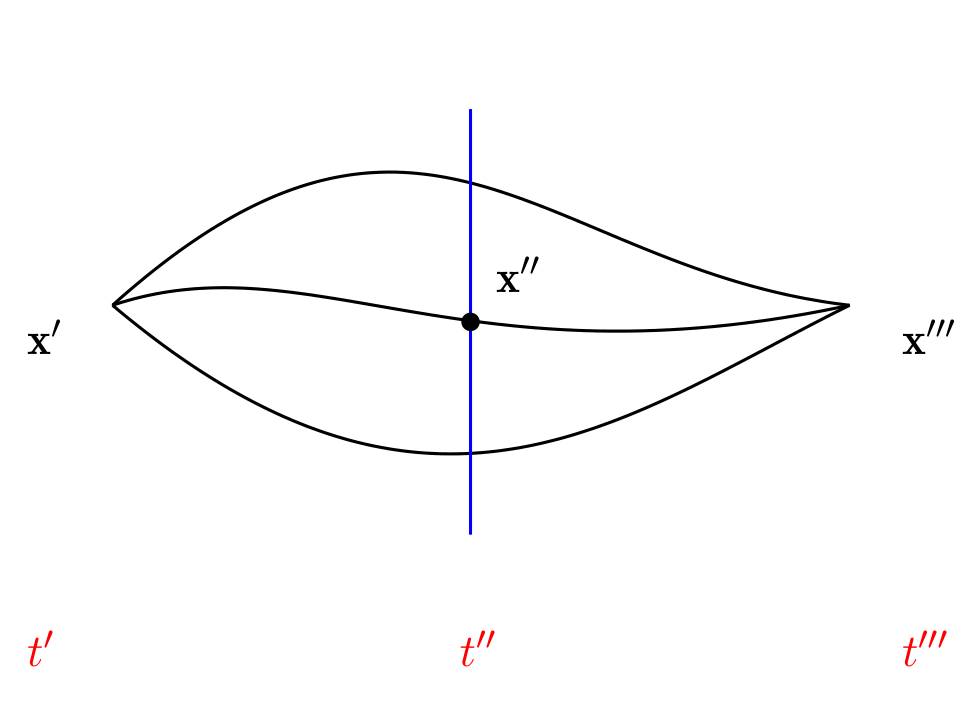
\includegraphics[width=0.62\textwidth]{figures/fig_p87_a.png}
\end{center}
% [图：原书 p.86，原图无题注]

把 $K(\mathbf{x}''',t''';\mathbf{x}',t')$ 看作从 $t'$ 时刻的 $\mathbf{x}'$ 到 $t'''$ 时刻的 $\mathbf{x}'''$ 的跃迁振幅，复合律说的是：这个跃迁振幅等于对中间时刻 $t''$ 处所有可能的 $\mathbf{x}''$ 的跃迁求和。

我们还可以进一步细分时间区间，取 $t_0=t'<t_1<t_2<\cdots<t_{N-1}<t_N=t''$。

\begin{center}
  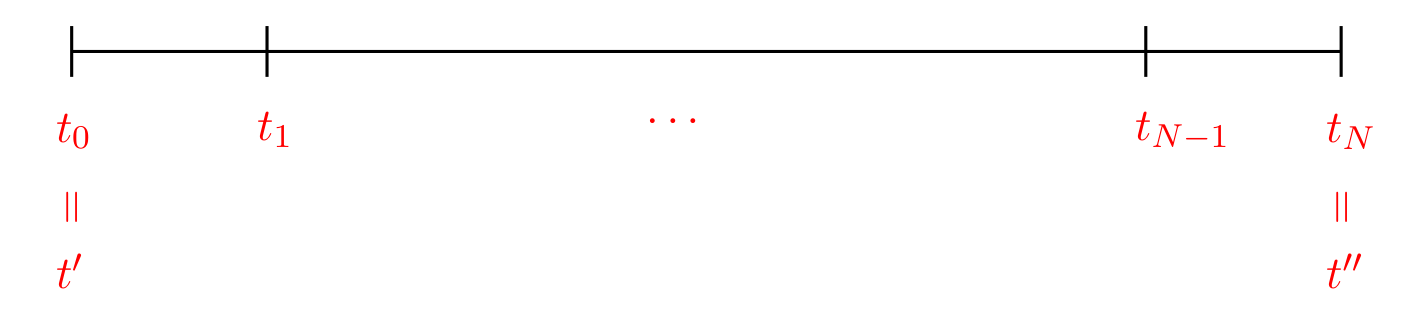
\includegraphics[width=0.64\textwidth]{figures/fig_p87_b.png}
\end{center}
% [图：原书 p.86，原图无题注]

% [原文 p.87]
同样的考虑给出复合律
\[
\begin{aligned}
K(\mathbf{x}'',t'';\mathbf{x}',t')
&=\int\rd^n\mathbf{x}_1\int\rd^n\mathbf{x}_2\cdots\int\rd^n\mathbf{x}_{N-1}\\
&\quad K(\mathbf{x}'',t'';\mathbf{x}_{N-1},t_{N-1})
\,K(\mathbf{x}_{N-1},t_{N-1};\mathbf{x}_{N-2},t_{N-2})\\
&\quad\cdots K(\mathbf{x}_1,t_1;\mathbf{x}',t').
\end{aligned}
\]

\begin{center}
  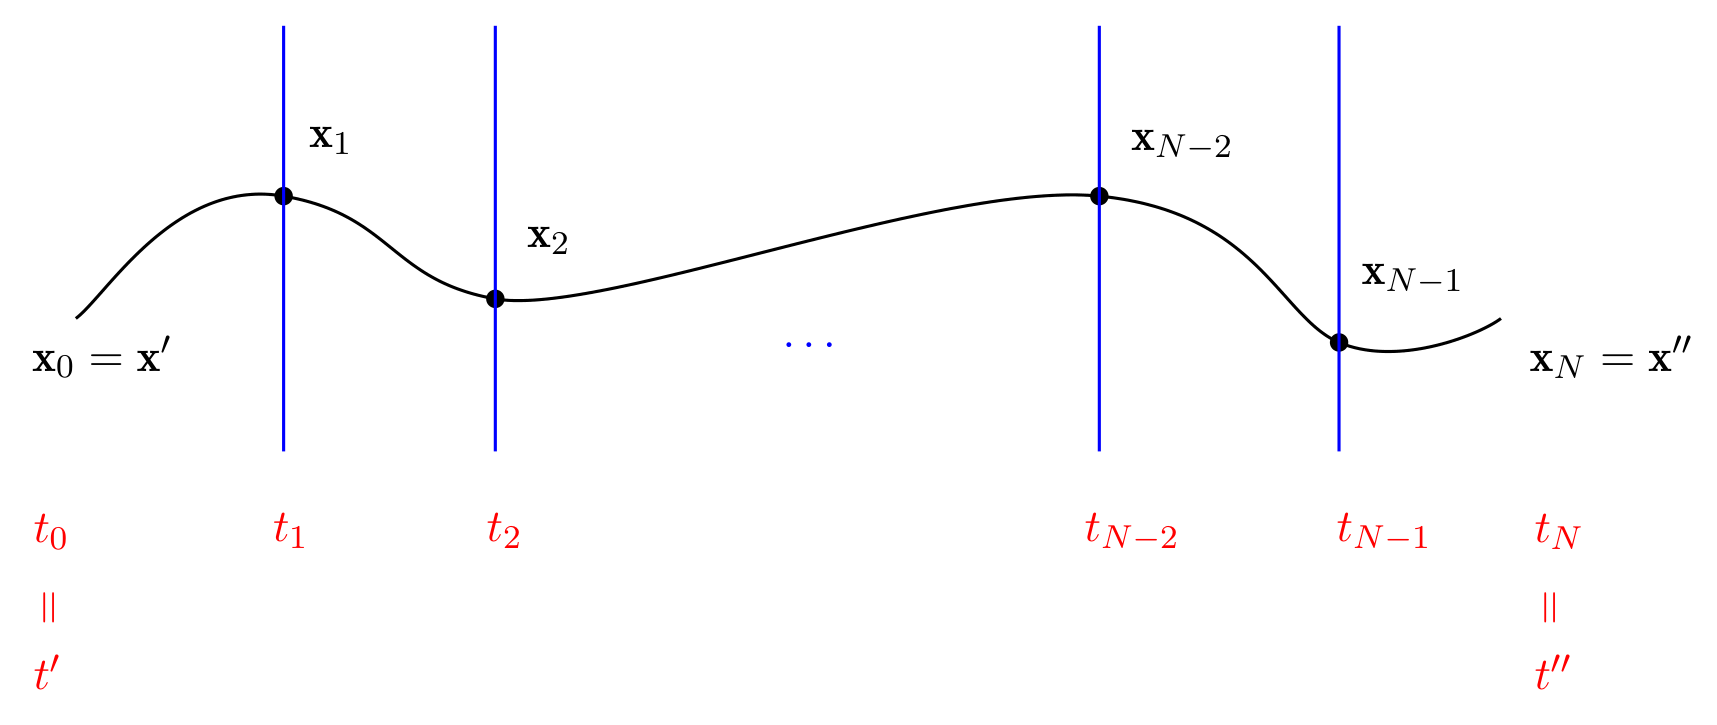
\includegraphics[width=0.75\textwidth]{figures/fig_p88_a.png}
\end{center}
% [图：原书 p.87，原图无题注]

这同样解释为对时刻 $t_1,t_2,\cdots,t_{N-1}$ 处所有可能的中间跃迁求和。

\subsection{路径积分}

现在可以把时间区间 $[t',t'']$ 细分，只要 $N$ 充分大
\[
t_0=t'<t_1<t_2<\cdots<t_{N-1}<t_N=t'',
\]
其中
\[
t_j=t'+j\epsilon,\qquad \epsilon=\frac{t''-t'}{N}.
\]
复合律给出
\[
K(\mathbf{x}'',t'';\mathbf{x}',t')
=\int\prod_{j=1}^{N-1}\rd^n\mathbf{x}_j\prod_{j=0}^{N-1}
K(\mathbf{x}_{j+1},t_{j+1};\mathbf{x}_j,t_j),
\qquad \mathbf{x}_0=\mathbf{x}',\ \mathbf{x}_N=\mathbf{x}''.
\]
代入前面关于短时间区间上积分核的结果，这近似为
\[
\simeq\left(\frac{m}{2\pi\hbar\ii\epsilon}\right)^{Nn/2}
\int\prod_{j=1}^{N-1}\rd^n\mathbf{x}_j\,
\ee^{\frac{\ii}{\hbar}\sum_{j=0}^{N-1}
\left[\frac m2\left(\frac{\mathbf{x}_{j+1}-\mathbf{x}_j}{\epsilon}\right)^2-V(\mathbf{x}_j)\right]\epsilon}.
\]
在 $N\to\infty$ 或 $\epsilon\to0$ 的极限下，这个积分预期趋于如下形式的费曼路径积分
\[
K(\mathbf{x}'',t'';\mathbf{x}',t')
=\int_{\mathbf{x}(t')=\mathbf{x}'}^{\mathbf{x}(t'')=\mathbf{x}''}
[D\mathbf{x}(t)]\,\ee^{\frac{\ii}{\hbar}\int_{t'}^{t''}
\left(\frac m2\dot{\mathbf{x}}^2-V(\mathbf{x})\right)\rd t},
\]
其中测度取为从 $t'$ 时刻的 $\mathbf{x}'$ 到 $t''$ 时刻的 $\mathbf{x}''$ 的路径空间上某个合适的测度。

% [原文 p.88]
\begin{center}
  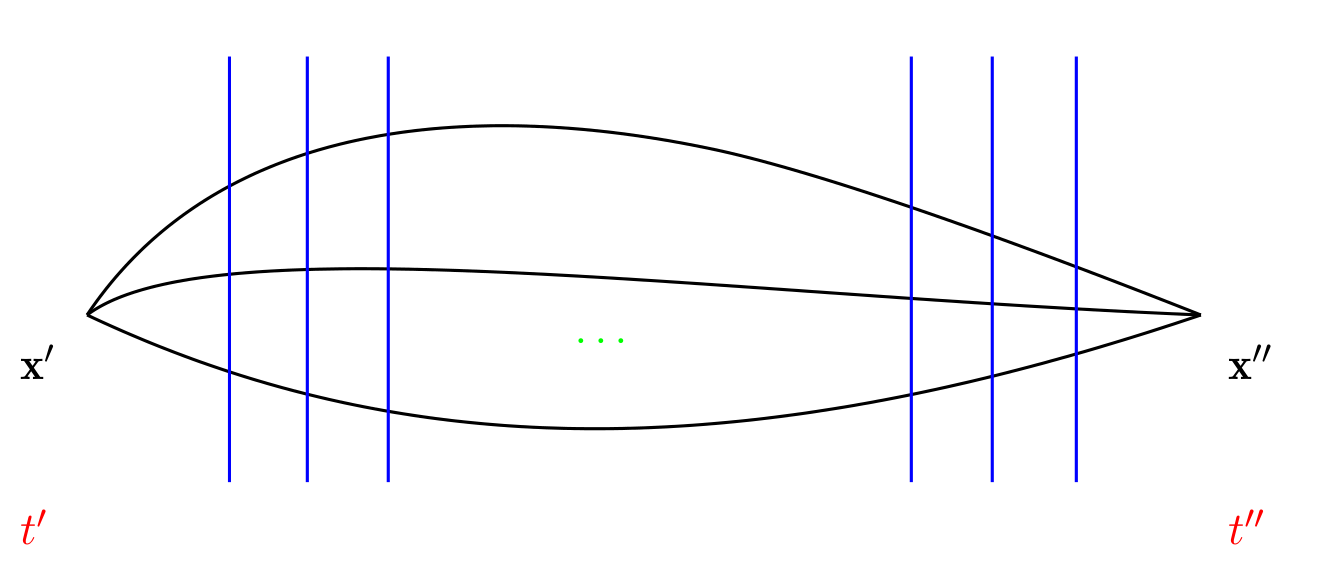
\includegraphics[width=0.66\textwidth]{figures/fig_p89_a.png}
\end{center}
% [图：原书 p.88，原图无题注]

注意
\[
S[\mathbf{x}(t)]=\int_{t'}^{t''}
\left(\frac m2\dot{\mathbf{x}}^2-V(\mathbf{x})\right)\rd t
\]
恰是经典作用量泛函。于是积分核 $K$ 也可写成
\[
K(\mathbf{x}'',t'';\mathbf{x}',t')
=\int_{\mathbf{x}(t')=\mathbf{x}'}^{\mathbf{x}(t'')=\mathbf{x}''}
[D\mathbf{x}(t)]\,\ee^{\frac{\ii}{\hbar}S[\mathbf{x}(t)]}.
\]
我们将在后续各节说明如何在适当意义下分析这个路径积分。

有了这个公式，费曼的路径积分可以理解为量子力学的\emph{拉格朗日表述}，它与传统的哈密顿算子方法相比提供了另一种视角。

\subsection{虚时间}

要得到数学性质更好的路径积分，更方便的做法是把时间作解析延拓
\[
t=-\ii\tau,\qquad \tau\in\R.
\]
这一解析延拓称为\emph{威克转动}（Wick rotation）。相应的路径积分称为\emph{欧氏路径积分}（Euclidean path integral）。记虚时间下的积分核为
\[
\begin{aligned}
K_E(\mathbf{x}'',\tau'';\mathbf{x}',\tau')
&:=K(\mathbf{x}'',-\ii\tau'';\mathbf{x}',-\ii\tau')
=\bra{\mathbf{x}''}\ee^{-\hat H(\tau''-\tau')/\hbar}\ket{\mathbf{x}'}\\
&=\int_{\mathbf{x}(\tau')=\mathbf{x}'}^{\mathbf{x}(\tau'')=\mathbf{x}''}
[D_E\mathbf{x}(\tau)]\,\ee^{-\frac1\hbar\int_{\tau'}^{\tau''}
\left(\frac m2\dot{\mathbf{x}}^2+V(\mathbf{x})\right)\rd\tau}.
\end{aligned}
\]
此时可以用条件维纳测度来定义 $[D_E\mathbf{x}(\tau)]$。在数学文献中，欧氏费曼路径积分的上述路径积分表示被称为\emph{费曼–卡茨公式}（Feynman-Kac formula）。

我们也将欧氏作用量记为
\[
S_E[\mathbf{x}(\tau)]=\int\left(\frac m2\dot{\mathbf{x}}^2+V(\mathbf{x})\right)\rd\tau.
\]
欧氏路径积分成为
\[
K_E(\mathbf{x}'',\tau'';\mathbf{x}',\tau')
=\int_{\mathbf{x}(\tau')=\mathbf{x}'}^{\mathbf{x}(\tau'')=\mathbf{x}''}
[D_E\mathbf{x}(\tau)]\,\ee^{-\frac1\hbar S_E[\mathbf{x}(\tau)]}.
\]
虚时间的物理意义是：欧氏核
\[
\rho(\mathbf{x}'',\mathbf{x}';\beta):=\bra{\mathbf{x}''}\ee^{-\beta\hat H}\ket{\mathbf{x}'}
\]
成为统计力学中的密度矩阵。

\takeaway{把时间区间切成 $N$ 段，反复用复合律积分，$N\to\infty$ 时得到费曼路径积分。作威克转动 $t=-\ii\tau$ 后每一步积分都是高斯型，欧氏路径积分有严格的维纳测度，欧氏核成为统计力学中的密度矩阵。}

% [原文 p.89]
\section{高斯路径积分}

\subsection{高斯积分}

回忆高斯积分公式
\[
\int_{\R}\rd x\,\ee^{-ax^2}=\sqrt{\frac{\pi}{a}},
\qquad a>0.
\]
这个高斯积分可以用解析延拓推广到虚相位 $a=-\ii\lambda$（见例 2.5.2）。它按如下方式取定 $\sqrt{\pi/a}=\sqrt{\ii\pi/\lambda}$ 的分支
\[
\int_{\R}\rd x\,\ee^{\ii\lambda x^2}
=\sqrt{\frac{\ii\pi}{\lambda}}
=\ee^{\frac{\ii\pi}{4}}\sgn\lambda\,\sqrt{\frac{\pi}{|\lambda|}},
\qquad \lambda\in\R-\{0\}.
\]
这可推广到 $n$ 维情形如下。

\begin{proposition}{2.3.1}
设 $A=(a_{ij})$ 是对称正定实矩阵。则
\[
\int_{\R^n}\rd^n\mathbf{x}\,\ee^{-\mathbf{x}^{\mathrm{t}}A\mathbf{x}}
=\frac{\pi^{n/2}}{\sqrt{\det A}}.
\tag{$*$}
\]
这里 $\mathbf{x}^{\mathrm{t}}A\mathbf{x}=\sum\limits_{i,j=1}^n a_{ij}x_ix_j$。更一般地，有
\[
\int_{\R^n}\rd^n\mathbf{x}\,
\ee^{-\mathbf{x}^{\mathrm{t}}A\mathbf{x}+\mathbf{J}^{\mathrm{t}}\cdot\mathbf{x}}
=\frac{\pi^{n/2}}{\sqrt{\det A}}\,
\ee^{\frac14\mathbf{J}^{\mathrm{t}}A^{-1}\mathbf{J}}.
\]
\end{proposition}

\begin{proof}
设
\[
A=P\begin{pmatrix}\lambda_1&&\\&\ddots&\\&&\lambda_n\end{pmatrix}P^{-1},
\]
其中 $P\in SO(n)$。考虑变量替换
\[
\mathbf{x}=P\mathbf{y}.
\]
由于 $P\in SO(n)$，这一变量替换的雅可比平凡，$\rd^n\mathbf{x}=\rd^n\mathbf{y}$。此外
\[
\mathbf{x}^{\mathrm{t}}A\mathbf{x}
=\mathbf{y}^{\mathrm{t}}P^{\mathrm{t}}AP\mathbf{y}
=\mathbf{y}^{\mathrm{t}}P^{-1}AP\mathbf{y}
=\mathbf{y}^{\mathrm{t}}\begin{pmatrix}\lambda_1&&\\&\ddots&\\&&\lambda_n\end{pmatrix}\mathbf{y}
=\lambda_1y_1^2+\lambda_2y_2^2+\cdots+\lambda_ny_n^2.
\]
因此
\[
\int_{\R^n}\rd^n\mathbf{x}\,\ee^{-\mathbf{x}^{\mathrm{t}}A\mathbf{x}}
=\int_{\R^n}\rd^n\mathbf{y}\,\ee^{-\sum\limits_{i=1}^n\lambda_iy_i^2}
=\prod_{i=1}^n\sqrt{\frac{\pi}{\lambda_i}}
=\frac{\pi^{n/2}}{\sqrt{\det A}}.
\]
带线性项 $\mathbf{J}^{\mathrm{t}}\cdot\mathbf{x}$ 的情形由配方可得。
\end{proof}

\begin{remark}{2.3.2}
这一结果可解析延拓到虚情形 $A=-\ii\Lambda$，且
\[
\int_{\R^n}\rd^n\mathbf{x}\,\ee^{\ii\mathbf{x}^{\mathrm{t}}\Lambda\mathbf{x}}
=\frac{\pi^{n/2}}{\sqrt{\det(-\ii\Lambda)}}
=\ee^{\frac{\ii\pi}{4}(n_+-n_-)}\,
\frac{\pi^{n/2}}{\sqrt{|\det\Lambda|}},
\]
其中 $n_+$、$n_-$ 分别是 $\Lambda$ 的正、负本征值个数。
\end{remark}

% [原文 p.90]
\subsection{zeta 函数正则化}

我们把高斯积分的想法用到路径积分上。为说明基本思路，从一维自由粒子这个最简单的例子入手，计算核
\[
K_0(x'',T;x',0)
=\int_{x(0)=x'}^{x(T)=x''}[Dx(t)]\,
\ee^{\frac{\ii}{\hbar}\int_0^T\left(\frac m2\dot x^2\right)\rd t}.
\]
记 $x_{cl}(t)$ 为从 $t=0$ 时刻的 $x'$ 到 $t=T$ 时刻的 $x''$ 的经典轨迹
\[
x_{cl}(t)=x'+\frac tT(x''-x').
\]
任何满足 $x(0)=x'$、$x(T)=x''$ 的路径 $x(t)$ 都可写成
\[
x(t)=x_{cl}(t)+\gamma(t),
\]
其中路径 $\gamma(t)$ 满足 $\gamma(0)=\gamma(T)=0$。可以把 $\gamma(t)$ 看作环绕经典轨迹 $x_{cl}(t)$ 的\emph{量子涨落}。

\begin{center}
  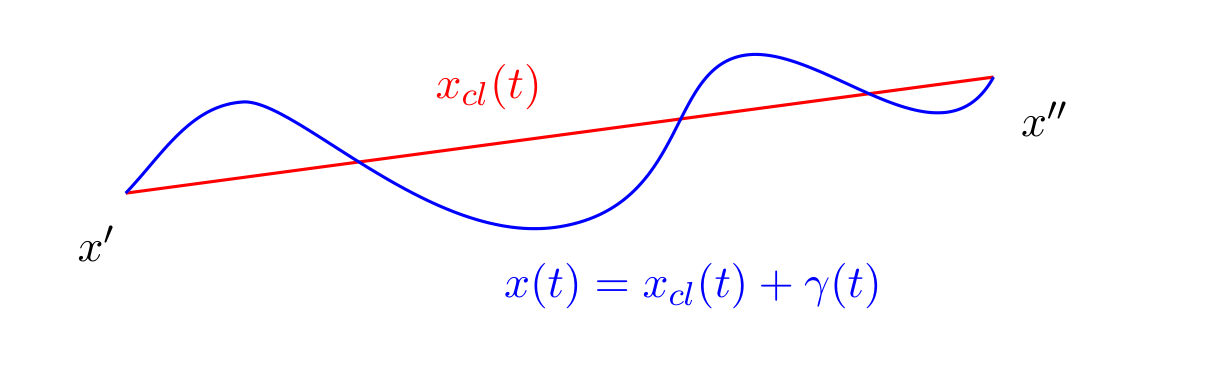
\includegraphics[width=0.68\textwidth]{figures/fig_p91_a.png}
\end{center}
% [图：原书 p.90，原图无题注]

由于经典轨迹 $x_{cl}(t)$ 是作用量的驻点，作用量泛函 $S[x]=S[x_{cl}+\gamma]$ 对 $\gamma$ 没有线性依赖。于是
\[
S[x]=\int_0^T\frac m2(\dot x_{cl}+\dot\gamma)^2\rd t
=\int_0^T\frac m2\dot x_{cl}^2\rd t+\int_0^T\frac m2\dot\gamma^2\rd t
=S[x_{cl}]+\int_0^T\frac m2\dot\gamma^2\rd t.
\]
这一点也可直接验证。第二项可以用分部积分写成
\[
\int_0^T\frac m2\dot\gamma^2\rd t
=-\frac m2\int_0^T\gamma\left(\frac{\rd^2}{\rd t^2}\right)\gamma\rd t.
\]
于是路径积分成为
\[
K(x'',T;x',0)=\ee^{\frac{\ii}{\hbar}S[x_{cl}]}
\int_{\gamma(0)=0}^{\gamma(T)=0}[D\gamma(t)]\,
\ee^{\frac{\ii m}{2\hbar}\int_0^T
\gamma\left(-\frac{\rd^2}{\rd t^2}\right)\gamma\rd t}.
\]
可见，关于 $\gamma(t)$ 的路径积分具有高斯积分的形式，只不过它是在满足 Dirichlet 边界条件 $\gamma(0)=\gamma(T)=0$ 的路径 $\gamma(t)$ 的无穷维空间上。与有限维高斯积分的类比是
\[
\begin{array}{ccc}
i & \longleftrightarrow & t\\
x_i & \longleftrightarrow & \gamma(t)\\
\sum\limits_i & \longleftrightarrow & \int\rd t\\
\int\prod\limits_i\rd x_i & \longleftrightarrow & \int[D\gamma(t)]
\end{array}
\]

% [原文 p.91]
记椭圆算子
\[
A=-\frac{\rd^2}{\rd t^2}.
\]
与有限维高斯积分比较，我们预期得到如下形式的结果
\[
\int_{\gamma(0)=0}^{\gamma(T)=0}[D\gamma(t)]\,
\ee^{\frac{\ii m}{2\hbar}\int_0^T
\gamma\left(-\frac{\rd^2}{\rd t^2}\right)\gamma\rd t}
=N(\det A)^{-\frac12},
\]
其中 $N$ 是某个待定的归一化常数。

我们需要给算子 $A$ 的行列式赋予意义。考虑 $A$ 在 Dirichlet 边界条件下的本征值问题
\[
A\gamma_m(t)=\lambda_m\gamma_m(t),\qquad \gamma_m(0)=\gamma_m(T)=0.
\]
由本征值问题的一般理论可知
\[
0<\lambda_1\le\lambda_2\le\cdots\le\lambda_m\le\cdots,
\qquad \lambda_m\to\infty\ \ (m\to+\infty),
\]
且 $\{\gamma_m(t)\}$ 构成满足 $\gamma(0)=\gamma(T)=0$ 的平方可积函数 $\gamma(t)$ 的希尔伯特空间的一组正交归一基。于是 $\det A$ 的朴素定义会是
\[
\det A\overset{?}{=}\prod_{m=1}^\infty\lambda_m.
\]
然而这个朴素乘积发散，因为 $m\to\infty$ 时 $\lambda_m\to\infty$。

幸运的是，可以用解析延拓绕开这一困难。对椭圆算子 $A$ 定义 zeta 函数
\[
\zeta_A(s):=\sum_{m=1}^\infty\frac1{\lambda_m^s},
\qquad s\in\C.
\]
已知 $\zeta_A(s)$ 的级数在 $\operatorname{Re}s$ 充分大时良定义，并可解析延拓到原点 $s=0$。于是
\[
\zeta_A'(0)\ \text{良定义}.
\]
直观上，导数公式
\[
\zeta_A'(s)=\sum_{m=1}^\infty\frac{-\ln\lambda_m}{\lambda_m^s},
\qquad \operatorname{Re}s\gg0
\]
提示朴素乘积 $\prod\limits_{m=1}^\infty\lambda_m$ 应由解析延拓定义为
\[
\text{「}\prod_{m=1}^\infty\lambda_m\text{」}:=\ee^{-\zeta_A'(0)}.
\]
于是可以定义算子 $A$ 的泛函行列式
\[
\det A:=\ee^{-\zeta_A'(0)}.
\]

% [原文 p.92]
我们来看它怎么起作用。$A$ 的本征函数与本征值容易求出
\[
\begin{cases}
\gamma_m(t)=c_m\sin\left(\dfrac{m\pi t}{T}\right), & c_m\ \text{为某常数},\\[2mm]
\lambda_m=\left(\dfrac{\pi m}{T}\right)^2. &
\end{cases}
\]
于是 zeta 函数 $\zeta_A(s)$ 为
\[
\zeta_A(s)=\sum_{m=1}^\infty\left(\frac{T}{\pi m}\right)^{2s}
=\left(\frac T\pi\right)^{2s}\zeta(2s),
\]
其中
\[
\zeta(s)=\sum_{m=1}^\infty\frac1{m^s}
\]
是黎曼 zeta 函数。利用已知结果
\[
\zeta(0)=-\frac12,\qquad \zeta'(0)=-\frac12\ln 2\pi,
\]
我们算出
\[
\zeta_A'(0)=2\ln\left(\frac T\pi\right)\zeta(0)+2\zeta'(0)
=-\ln\left(\frac T\pi\right)-\ln 2\pi=-\ln 2T.
\]
于是
\[
\det A=\ee^{-\zeta_A'(0)}=2T.
\]
把它代入路径积分，得到
\[
K_0(x'',T;x',0)=\frac{N}{\sqrt{2T}}\,\ee^{\frac{\ii}{\hbar}S[x_{cl}]}
=\frac{N}{\sqrt{2T}}\,\ee^{\frac{\ii m(x''-x')^2}{2\hbar T}}.
\]
这与我们此前对自由粒子得到的结果一致，归一化常数为
\[
N=\left(\frac{m}{\pi\ii\hbar}\right)^{\frac12}.
\]
这个结果提示：对一维的一般椭圆算子 $A$，有高斯路径积分
\[
\int_{\gamma(0)}^{\gamma(T)}[D\gamma(t)]\,
\ee^{\frac{\ii m}{2\hbar}\int_0^T\gamma A\gamma\rd t}
=\left(\frac{m}{\pi\ii\hbar}\right)^{\frac12}(\det A)^{-\frac12},
\]
其中 $\det A$ 通过 zeta 函数 $\zeta_A(s)$ 的解析延拓定义
\[
\det A:=\ee^{-\zeta_A'(0)}.
\]
这个方法称为\emph{zeta 函数正则化}（zeta function regularization）。

\takeaway{高斯积分可解析延拓到虚相位；对无穷维的高斯路径积分，算子行列式用 zeta 函数正则化定义：$\det A:=\ee^{-\zeta_A'(0)}$。据此算出一维自由粒子的核，并自然定出归一化常数 $N$。}

% [原文 p.93]
\section{谐振子}

\subsection{积分核}

作为路径积分方法的例证，我们重温一维谐振子的例子。哈密顿算子为
\[
\hat H=\frac1{2m}\hat p^2+\frac m2\omega^2\hat x^2.
\]
我们计算积分核
\[
K(x'',T;x',0)=\bra{x''}\ee^{-\ii\hat HT/\hbar}\ket{x'}
=\int_{x(0)=x'}^{x(T)=x''}[Dx(t)]\,
\ee^{\frac{\ii}{\hbar}\int_0^T\left(\frac m2\dot x^2-\frac m2\omega^2x^2\right)\rd t}.
\]
作用量泛函为
\[
S[x(t)]=\int_0^T\left(\frac m2\dot x^2-\frac m2\omega^2x^2\right)\rd t.
\]
设 $x_{cl}(t)$ 是满足经典运动方程的经典轨迹
\[
\ddot x_{cl}(t)=-\omega^2x_{cl}(t),
\]
边界条件为 $x_{cl}(0)=x'$、$x_{cl}(T)=x''$。其解为
\[
x_{cl}(t)=\frac{\sin\omega(T-t)}{\sin\omega T}\,x'
+\frac{\sin\omega t}{\sin\omega T}\,x''.
\]
任何满足 $x(0)=x'$、$x(T)=x''$ 的路径 $x(t)$ 都可分解为
\[
x(t)=x_{cl}(t)+\gamma(t),
\]
其中 $\gamma(t)$ 是满足边界条件
\[
\gamma(0)=\gamma(T)=0
\]
的任意路径。

作用量成为
\[
\begin{aligned}
S[x(t)]&=S[x_{cl}(t)+\gamma(t)]\\
&=S[x_{cl}(t)]+\int_0^T\left(\frac m2\dot\gamma^2-\frac m2\omega^2\gamma^2\right)\rd t\\
&=S[x_{cl}(t)]+\frac m2\int_0^T\gamma\left(-\frac{\rd^2}{\rd t^2}-\omega^2\right)\gamma\rd t\\
&=S[x_{cl}(t)]+\frac m2\int_0^T\gamma A\gamma\rd t.
\end{aligned}
\]
这里 $A$ 是椭圆算子
\[
A=-\frac{\rd^2}{\rd t^2}-\omega^2.
\]
路径积分是高斯型的，因此
\[
\begin{aligned}
K(x'',T;x',0)&=\ee^{\frac{\ii}{\hbar}S[x_{cl}(t)]}
\int_{\gamma(0)=0}^{\gamma(T)=0}[D\gamma(t)]\,
\ee^{\frac{\ii m}{2\hbar}\int_0^T\gamma A\gamma\rd t}\\
&=\left(\frac{m}{\pi\ii\hbar}\right)^{\frac12}
\ee^{\frac{\ii}{\hbar}S[x_{cl}(t)]}(\det A)^{-\frac12}.
\end{aligned}
\]

% [原文 p.94]
我们按 §2.3.2 的做法，用 zeta 函数正则化计算 $\det A$。本征函数与本征值为
\[
\begin{cases}
\gamma_m(t)=c_m\sin\left(\dfrac{m\pi t}{T}\right), & c_m\ \text{为某常数},\\[2mm]
\lambda_m=\left(\dfrac{\pi m}{T}\right)^2-\omega^2
=\left(\dfrac{\pi m}{T}\right)^2\left[1-\left(\dfrac{\omega T}{\pi m}\right)^2\right]. &
\end{cases}
\]
于是朴素地得到
\[
\det A=\prod_{m=1}^\infty\left[\left(\frac{\pi m}{T}\right)^2
\left(1-\left(\frac{\omega T}{\pi m}\right)^2\right)\right]
=\prod_{m=1}^\infty\left(\frac{\pi m}{T}\right)^2
\prod_{m=1}^\infty\left[1-\left(\frac{\omega T}{\pi m}\right)^2\right].
\]
第一项用黎曼 zeta 函数正则化，§2.3.2 已算出
\[
\prod_{m=1}^\infty\left(\frac{\pi m}{T}\right)^2=2T.
\]
第二项收敛。事实上，利用
\[
\prod_{m=1}^\infty\left[1-\left(\frac{z}{\pi m}\right)^2\right]=\frac{\sin z}{z},
\]
我们有
\[
\prod_{m=1}^\infty\left[1-\left(\frac{\omega T}{\pi m}\right)^2\right]
=\frac{\sin\omega T}{\omega T}.
\]
因此
\[
\det A=(2T)\left(\frac{\sin\omega T}{\omega T}\right)=\frac{2\sin\omega T}{\omega}.
\]
费曼核 $K$ 成为
\[
K(x'',T;x',0)=\left(\frac{m\omega}{2\pi\ii\hbar\sin\omega T}\right)^{\frac12}
\ee^{\frac{\ii}{\hbar}S[x_{cl}(t)]}.
\]
经典轨迹的作用量为
\[
\begin{aligned}
S[x_{cl}(t)]
&=\frac m2\int_0^T\left(\dot x_{cl}^2-\omega^2x_{cl}^2\right)\rd t\\
&=\frac m2\,x_{cl}\dot x_{cl}\Big|_0^T
-\frac m2\int_0^T\left(x_{cl}\ddot x_{cl}+\omega^2x_{cl}^2\right)\rd t\\
&=\frac m2\left(x_{cl}(T)\dot x_{cl}(T)-x_{cl}(0)\dot x_{cl}(0)\right)\\
&=\frac m2\left(-\frac{\omega}{\sin\omega T}x'
+\frac{\omega\cos\omega T}{\sin\omega T}x''\right)x''
-\frac m2\left(-\frac{\omega\cos\omega T}{\sin\omega T}x'
+\frac{\omega}{\sin\omega T}x''\right)x'\\
&=\frac{m\omega}{2\sin\omega T}\left[\left((x')^2+(x'')^2\right)\cos\omega T-2x'x''\right].
\end{aligned}
\]
我们得到量子谐振子积分核的最终结果
\[
K(x'',T;x',0)=\left(\frac{m\omega}{2\pi\ii\hbar\sin\omega T}\right)^{\frac12}
\ee^{\frac{\ii m\omega}{2\hbar}\left[\left((x')^2+(x'')^2\right)\cot\omega T
-\frac{2x'x''}{\sin\omega T}\right]}.
\]

% [原文 p.95]
\subsection{配分函数}

我们想把谐振子的费曼核与 §1.7 关于能谱的结果作比较。纽带是由
\[
\Tr\ee^{-\beta\hat H}
\]
定义的配分函数。我们将用两种不同方法计算它。

第一种方法是借助能谱计算配分函数
\[
\Tr\ee^{-\beta\hat H}
=\sum_{n=0}^\infty\ee^{-\beta E_n}
=\sum_{n=0}^\infty\ee^{-\beta\left(n+\frac12\right)\hbar\omega}
=\frac{\ee^{-\frac12\beta\hbar\omega}}{1-\ee^{-\beta\hbar\omega}}
=\frac{1}{2\sinh(\beta\hbar\omega/2)}.
\]
第二种方法是用费曼核计算配分函数。考虑虚时间
\[
T=-\ii\tau
\]
与欧氏积分核
\[
K_E(x'',\tau;x',0)=K(x'',-\ii\tau;x',0)
=\bra{x''}\ee^{-\hat H\tau/\hbar}\ket{x'}.
\]
配分函数作为迹也可写成
\[
\Tr\ee^{-\beta\hat H}
=\int\rd x\,\bra{x}\ee^{-\beta\hat H}\ket{x}
=\int\rd x\,K_E(x,\beta\hbar;x,0)
=\int\rd x\,K(x,-\ii\beta\hbar;x,0).
\]
代入费曼核的显式结果，
\[
\begin{aligned}
\Tr\ee^{-\beta\hat H}
&=\int_{\R}\rd x\left(\frac{m\omega}{2\pi\hbar\sinh(\beta\omega\hbar)}\right)^{\frac12}
\ee^{-\frac{2m\omega\sinh^2(\beta\omega\hbar/2)}{\hbar\sinh(\beta\omega\hbar)}x^2}\\
&=\left(\frac{m\omega}{2\pi\hbar\sinh(\beta\omega\hbar)}
\cdot\frac{\pi\hbar\sinh(\beta\omega\hbar)}{2m\omega\sinh^2(\beta\omega\hbar/2)}\right)^{\frac12}\\
&=\frac{1}{2\sinh(\beta\hbar\omega/2)}.
\end{aligned}
\]
这与能谱计算的结果相同，而且走了一条不平凡的路。物理是自洽的！

\takeaway{把路径写成经典轨迹加涨落，谐振子的作用量化为高斯型；用 zeta 函数正则化算出 $\det A$，得到传播子的显式表达式。再取迹并作虚时间延拓，两种算法给出同一个配分函数 $1/(2\sinh(\beta\hbar\omega/2))$。}

\section{渐近方法}

本节回顾振荡积分渐近分析的一些基本工具。这将帮助我们在后续各节处理路径积分，得到量子力学中的半经典结果。这个题材相当经典，但很容易陷入技术性讨论。我们反过来选择直观的路子，用例子说明基本想法，目的是为后面操作路径积分作铺垫。

% [原文 p.96]
\subsection{拉普拉斯方法}

我们从拉普拉斯方法说起，它用来分析如下形式的积分
\[
\int_a^b\ee^{-\lambda f(x)}\rd x,
\]
并给出 $\lambda\to+\infty$ 时的首阶渐近近似。为简单起见，假设
\begin{itemize}
  \item $[a,b]$ 是有限区间。若对 $f$ 在无穷端点附近再加些温和假设，讨论可推广到 $a=-\infty$ 或 $b=+\infty$（或两者）的情形。
  \item $f$ 是 $[a,b]$ 上二次连续可微函数，在内部一点 $x_0\in(a,b)$ 取得唯一全局极小，且
  \[
  f''(x_0)>0.
  \]
\end{itemize}
在这些假设下，拉普拉斯方法表明
\[
\lim_{\lambda\to\infty}
\frac{\int_a^b\ee^{-\lambda f(x)}\rd x}
{\ee^{-\lambda f(x_0)}\sqrt{\dfrac{2\pi}{\lambda f''(x_0)}}}=1.
\tag{$*$}
\]
我们通常把它写成渐近近似
\[
\int_a^b\ee^{-\lambda f(x)}\rd x
\simeq\ee^{-\lambda f(x_0)}\sqrt{\frac{2\pi}{\lambda f''(x_0)}},
\qquad \lambda\to+\infty.
\]
用拉普拉斯方法得出近似公式 $(*)$ 的想法是：在 $\lambda\to+\infty$ 的极限下，积分由全局极小 $x_0$ 的小邻域上的
\[
\int_{x_0-\epsilon}^{x_0+\epsilon}\ee^{-\lambda f(x)}\rd x
\]
主导。若在 $x_0$ 处作泰勒展开（注意 $f'(x_0)=0$）
\[
f(x)=f(x_0)+\frac{f''(x_0)}{2}(x-x_0)^2+O\left((x-x_0)^3\right),
\]
并作变量替换
\[
x=x_0+\frac{y}{\sqrt{\lambda}},
\]
则有
\[
\begin{aligned}
\int_{x_0-\epsilon}^{x_0+\epsilon}\ee^{-\lambda f(x)}\rd x
&=\frac{\ee^{-\lambda f(x_0)}}{\sqrt{\lambda}}
\int_{-\sqrt{\lambda}\epsilon}^{\sqrt{\lambda}\epsilon}
\ee^{-\frac{f''(x_0)}{2}y^2+O\left(\frac1{\sqrt{\lambda}}\right)}\rd y\\
&\simeq\frac{\ee^{-\lambda f(x_0)}}{\sqrt{\lambda}}
\int_{-\infty}^{+\infty}\ee^{-\frac{f''(x_0)}{2}y^2}\rd y
\qquad \lambda\to+\infty\\
&=\ee^{-\lambda f(x_0)}\sqrt{\frac{2\pi}{\lambda f''(x_0)}}.
\end{aligned}
\]

% [原文 p.97]
\begin{center}
  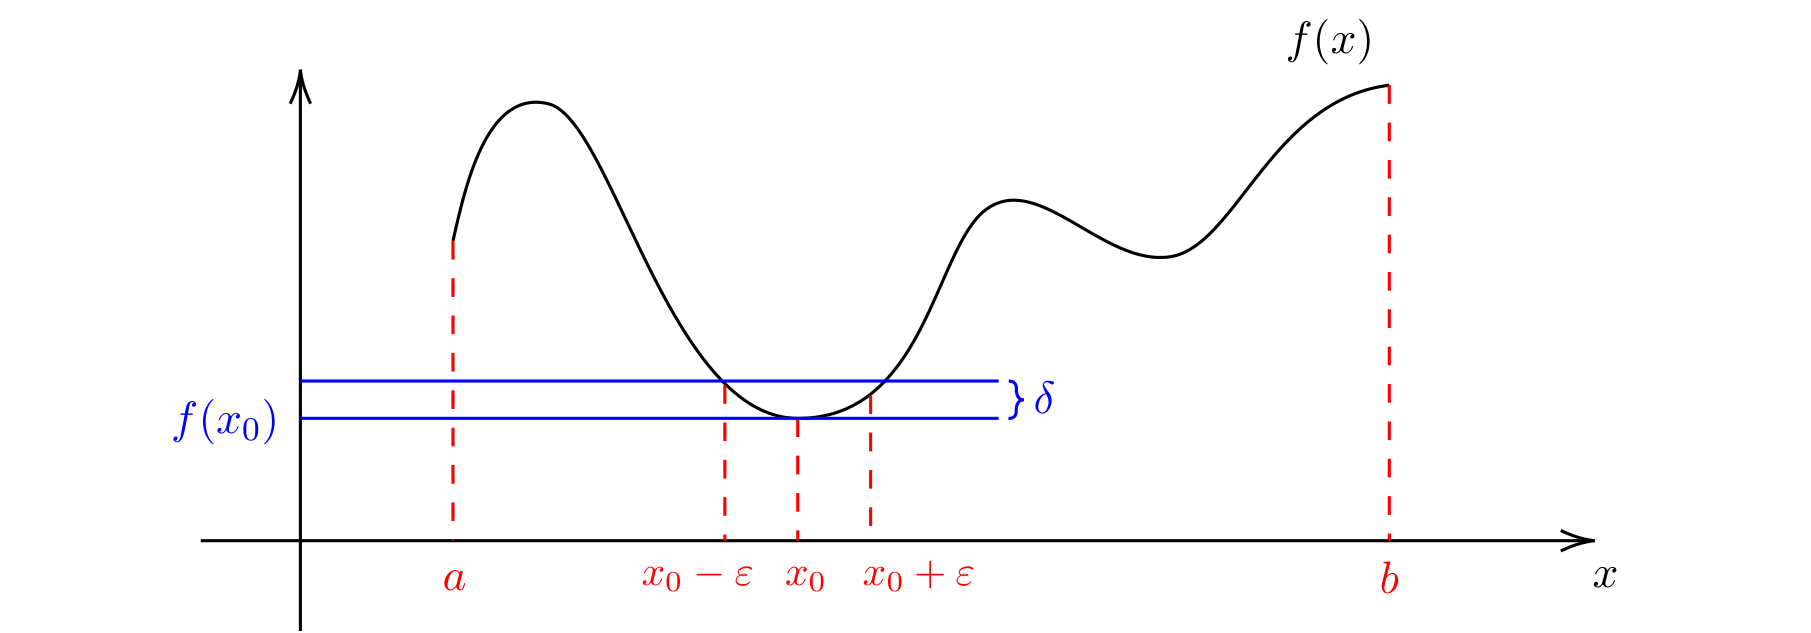
\includegraphics[width=0.75\textwidth]{figures/fig_p98_a.png}
\end{center}
% [图：原书 p.97，原图无题注]

在 $[x_0-\epsilon,x_0+\epsilon]$ 之外，
\[
\ee^{-\lambda f(x)}=\ee^{-\lambda f(x_0)}O\left(\ee^{-\lambda\delta}\right).
\]
$(*)$ 的证明基本上就是把上面的想法通过仔细的误差分析实现出来。若对 $f$ 在无穷端点附近另加一些温和假设，这个渐近公式也可推广到 $a=-\infty$ 或 $b=+\infty$（或两者）的情形。

上面的讨论还可推广到
\[
\int_a^b g(x)\ee^{-\lambda f(x)}\rd x,
\]
其中 $g(x)$ 为正。此时
\[
\int_a^b g(x)\ee^{-\lambda f(x)}\rd x
\simeq g(x_0)\ee^{-\lambda f(x_0)}\sqrt{\frac{2\pi}{\lambda f''(x_0)}},
\qquad \lambda\to+\infty.
\]

\begin{example}{2.5.1}
考虑 $\Gamma$ 函数
\[
\Gamma(s)=\int_0^{+\infty}\rd x\,x^{s-1}\ee^{-x}.
\]
我们考虑它在 $s\to+\infty$ 时的渐近行为。上面的讨论可推广到这一情形。把它改写为
\[
\Gamma(s)=(s-1)^s\int_0^{+\infty}\rd x\,\ee^{-(x-\ln x)\lambda},
\qquad \lambda=s-1,
\]
于是本例中 $f(x)=x-\ln x$。极小在点
\[
f'(x_0)=1-\frac1{x_0}=0
\quad\Longrightarrow\quad
x_0=1
\]
取得。由此得到一渐近近似
\[
\begin{aligned}
\Gamma(s)&\simeq(s-1)^s\sqrt{\frac{2\pi}{\lambda f''(x_0)}}\,
\ee^{-\lambda f(x_0)}\\
&=\sqrt{2\pi}\,(s-1)^{s-\frac12}\ee^{1-s}\\
&=\sqrt{\frac{2\pi}{s}}\,\sqrt{\frac{s}{s-1}}\,s^s
\left(1-\frac1s\right)^s\ee^{1-s}\\
&\simeq\sqrt{\frac{2\pi}{s}}\left(\frac se\right)^s
\qquad (s\to+\infty).
\end{aligned}
\]
这就是著名的\emph{斯特林公式}（Stirling's formula）。
\end{example}

% [原文 p.98]
上面的讨论可推广到 $n$ 维情形
\[
\int_\Gamma\ee^{-\lambda f(\mathbf{x})}\rd^n\mathbf{x},
\qquad \mathbf{x}=(x^1,\cdots,x^n).
\]
设 $f(\mathbf{x})$ 在积分区域内部有唯一全局极小 $\mathbf{x}_0$，且 黑塞矩阵 $H_f=(\pa_{x^i}\pa_{x^j}f)$ 在 $\mathbf{x}_0$ 处正定
\[
H_f(\mathbf{x}_0)>0.
\]
作类似的考虑，在 $\lambda\to+\infty$ 的极限下，主要贡献来自 $\mathbf{x}_0$ 的近邻，首阶近似由高斯积分给出
\[
\ee^{-\lambda f(\mathbf{x}_0)}
\int_{\R^n}\rd^n\mathbf{x}\,
\ee^{-\frac\lambda2\mathbf{x}^{\mathrm{t}}H_f(\mathbf{x}_0)\mathbf{x}}
=\left(\frac{2\pi}{\lambda}\right)^{\frac n2}
\frac{1}{\sqrt{\det(H_f(\mathbf{x}_0))}}\,\ee^{-\lambda f(\mathbf{x}_0)}.
\]
于是拉普拉斯方法给出
\[
\int\rd^n\mathbf{x}\,g(\mathbf{x})\ee^{-\lambda f(\mathbf{x})}
\simeq\left(\frac{2\pi}{\lambda}\right)^{\frac n2}
\frac{g(\mathbf{x}_0)}{\sqrt{\det(H_f(\mathbf{x}_0))}}\,
\ee^{-\lambda f(\mathbf{x}_0)},
\qquad \lambda\to+\infty.
\]

\subsection{最速下降法}

拉普拉斯方法可推广到如下形式的复振荡积分
\[
I(\lambda)=\int_C\rd z\,g(z)\ee^{-\lambda f(z)},
\]
其中 $f(z)$、$g(z)$ 是 $z$ 的解析函数。由柯西积分公式，这个复积分在 $C$ 的连续形变下不变（$C$ 的无穷远端需满足适当边界条件）。这样，只要把围道适当变形，就能作解析延拓与渐近分析。

\begin{example}{2.5.2}
考虑如下积分
\[
\int_C\ee^{\ii z^2}\rd z.
\]
它可看作标准高斯积分
\[
\int_{\R}\ee^{-\lambda x^2}\rd x,\qquad \lambda>0
\]
的解析延拓。从 $\lambda>0$ 延拓到 $\lambda=-\ii$，只需选取合适的围道：

\begin{center}
\begin{tikzpicture}[scale=1.0,>=Stealth]
  \draw[->] (-2.6,0) -- (2.6,0) node[right] {$x$};
  \draw[->] (0,-1.7) -- (0,1.7) node[above] {$y$};
  \draw[blue,thick] (-2.3,-0.62) -- (2.3,0.62);
  \draw[->,blue,thick] (-2.3,-0.62) -- (-2.05,-0.553);
  \draw[->,blue,thick] (1.2,0.323) -- (1.45,0.39);
  \draw (0.5,0) arc (0:15:0.5);
  \node at (0.78,0.11) {$\theta$};
  \node[blue] at (2.45,0.92) {$C_\theta$};
  \node at (2.15,1.35) {$\theta>0$ 且很小};
\end{tikzpicture}
\end{center}
% [图：原书 p.98，本图按原文重绘，图内标注已译为中文；原图无题注]

% [原文 p.99]
则
\[
I(\lambda)=\int_{C_\theta}\ee^{-\lambda z^2}\rd z
\]
在 $\operatorname{Re}\lambda\ge0$、$\operatorname{Im}\lambda\le0$、$\lambda\ne0$ 时收敛。于是 $I(\lambda)$ 给出从 $\lambda\in\R_{>0}$ 到 $\lambda\in\ii\R_{<0}$ 的解析延拓。特别地
\[
I(-\ii)=\int_{C_\theta}\ee^{\ii z^2}\rd z
=\int_{C_{\frac\pi4}}\ee^{\ii z^2}\rd z
=\ee^{\frac\pi4\ii}\int_{-\infty}^{+\infty}\ee^{-u^2}\rd u
=\ee^{\frac\pi4\ii}\sqrt{\pi}.
\]
类似地，若把围道顺时针形变，则得到从 $\lambda>0$ 到 $\lambda=\ii$ 的解析延拓
\[
\int_{C_{-\frac\pi4}}\ee^{-\ii z^2}\rd z=\ee^{-\frac\pi4\ii}\sqrt{\pi}.
\]
这就解释了 §2.3.1 中关于高斯积分的讨论。
\end{example}

一般地，最速下降法就是把围道 $C$ 形变到一条曲线，沿它 $|\ee^{-f(z)}|$ 衰减最快。为看清这样的围道长什么样，记
\[
f(z)=u(x,y)+\ii v(x,y),\qquad z=x+\ii y.
\]
于是 $u=\operatorname{Re}f$、$v=\operatorname{Im}f$。最速下降曲线应沿 $u$ 的梯度方向，因为
\[
|\ee^{-f}|=\ee^{-u}.
\]
由于 $f(z)$ 解析，$u$、$v$ 满足柯西–黎曼方程
\[
\pa_xu=\pa_yv,\qquad \pa_yu=-\pa_xv.
\]
由此可知
\[
\nabla u\cdot\nabla v=\pa_xu\,\pa_xv+\pa_yu\,\pa_yv=0.
\]
换言之，$\nabla v$ 与 $u$ 的梯度方向垂直，所以最速下降曲线落在 $v$ 的某条水平集上。这引出如下策略：把围道 $C$ 形变为围道 $C'$，使得
\begin{itemize}
  \item[①] $\operatorname{Im}f$ 沿 $C'$ 为常数；
  \item[②] $C'$ 经过一个或多个满足
  \[
  f'(z)=0
  \]
  的点。
\end{itemize}
这些点称为\emph{鞍点}（saddle point）。它们也是 $\operatorname{Re}f$ 沿 $C'$ 的临界点。于是
\[
I(\lambda)=\int_{C'}\rd z\,g(z)\ee^{-\lambda f(z)}
=\ee^{-\ii\lambda\operatorname{Im}f}\int_{C'}g(z)\ee^{-\lambda\operatorname{Re}f}\rd z,
\]
我们就可以应用拉普拉斯方法了。

设 $C'$ 上有一个非退化鞍点 $z_0$，且它是 $C'$ 上的全局极小。非退化鞍点的条件是
\[
f'(z_0)=0,\qquad f''(z_0)\ne0.
\]

% [原文 p.100]
于是用高斯积分作局部计算给出
\[
\int_{C'}g(z)\ee^{-\lambda f(z)}\rd z
\simeq\sqrt{\frac{2\pi}{\lambda f''(z_0)}}\,g(z_0)\ee^{-\lambda f(z_0)},
\qquad \lambda\to+\infty.
\]
$n$ 维复积分也有类似结果。高斯积分中平方根的分支由解析延拓确定，如上面的例子所示。

\begin{example}{2.5.3}
考虑高斯积分
\[
\int_C\ee^{\ii\lambda z^2}\rd z,\qquad \lambda>0.
\]
此时 $f(z)=-\ii z^2$，且
\[
\operatorname{Re}f=2xy,\qquad \operatorname{Im}f=y^2-x^2.
\]
最速下降围道为

\begin{center}
  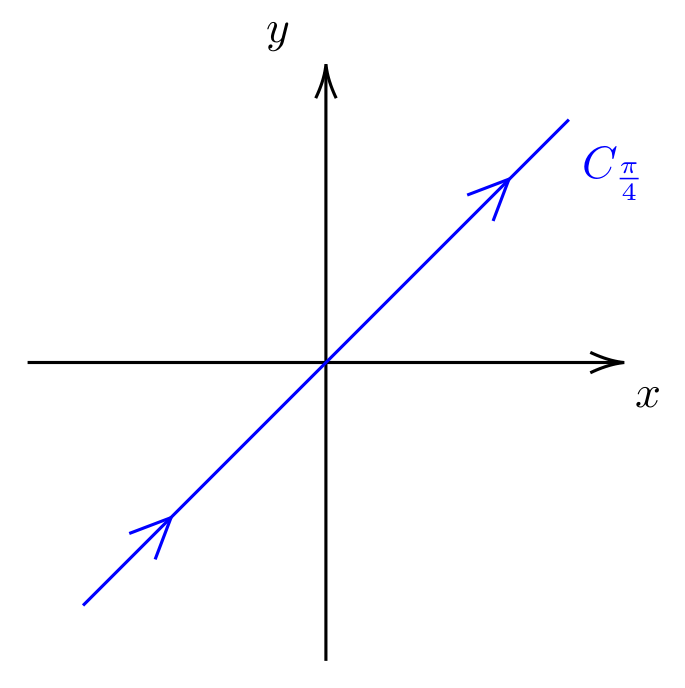
\includegraphics[width=0.34\textwidth]{figures/fig_p101_a.png}
\end{center}
% [图：原书 p.100，原图无题注]
\end{example}

\subsection{莫尔斯流}

具体地说，最速下降曲线可以用莫尔斯理论构造。我们沿用文献 [60] 的讲法，就本文情形说明基本想法。考虑如下流方程
\[
\begin{cases}
\dfrac{\rd z}{\rd u}=-\overline{f'(z)}\\[2mm]
\lim\limits_{u\to-\infty}z(u)=\text{鞍点}
\end{cases}
\]
其中 $u\in\R$ 是流的实参数。沿流有
\[
\frac{\rd f(z)}{\rd u}=-|f'(z)|^2.
\]
所以 $\operatorname{Im}f$ 为常数，$\operatorname{Re}f$ 沿流递减，由此得到最速下降曲线。

\begin{example}{2.5.4}
来看一个例子
\[
\int_C\ee^{\lambda f(z)},\qquad f(z)=\frac{\alpha z^2}{2},
\quad \alpha\in\C^*,\ \lambda>0.
\]

% [原文 p.101]
鞍点在 $z=0$ 处。最速下降曲线 $C$ 满足
\[
\operatorname{Im}f=0,
\qquad\text{且}\quad
\operatorname{Re}f\to-\infty\ \ \text{沿}\ \partial C.
\]
这样的曲线 $C$ 可以通过解流方程构造
\[
\begin{cases}
\dfrac{\rd z}{\rd u}=-\overline{f'(z)}=-\bar\alpha\bar z\\[2mm]
\lim\limits_{u\to-\infty}z(u)=0
\end{cases}
\]
设 $\alpha=A\ee^{\ii\theta}$，$A>0$。有两个指向相反方向的解
\[
z(u)=\pm\ee^{Au}\ee^{\frac{\ii}{2}(\pi-\theta)}.
\]
相应的解如图所示（箭头表示流的方向）

\begin{center}
  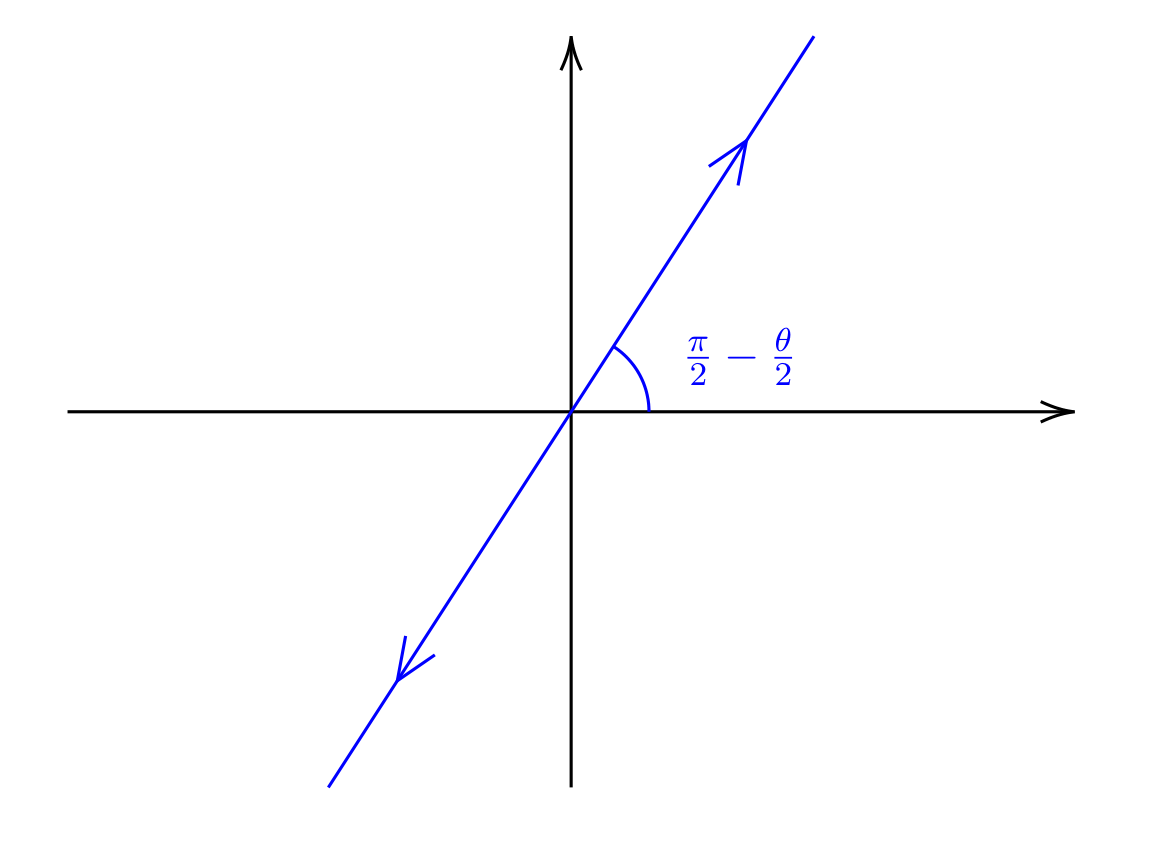
\includegraphics[width=0.42\textwidth]{figures/fig_p102_a.png}
\end{center}
% [图：原书 p.101，原图无题注]

解沿图中所示角度的方向流动
\[
\frac\pi2-\frac\theta2=\frac\pi2-\frac12\operatorname{Arg}\left(f''(0)\right).
\]
适当地选定定向后，这两支流合起来构成曲线 $C$。

\begin{center}
  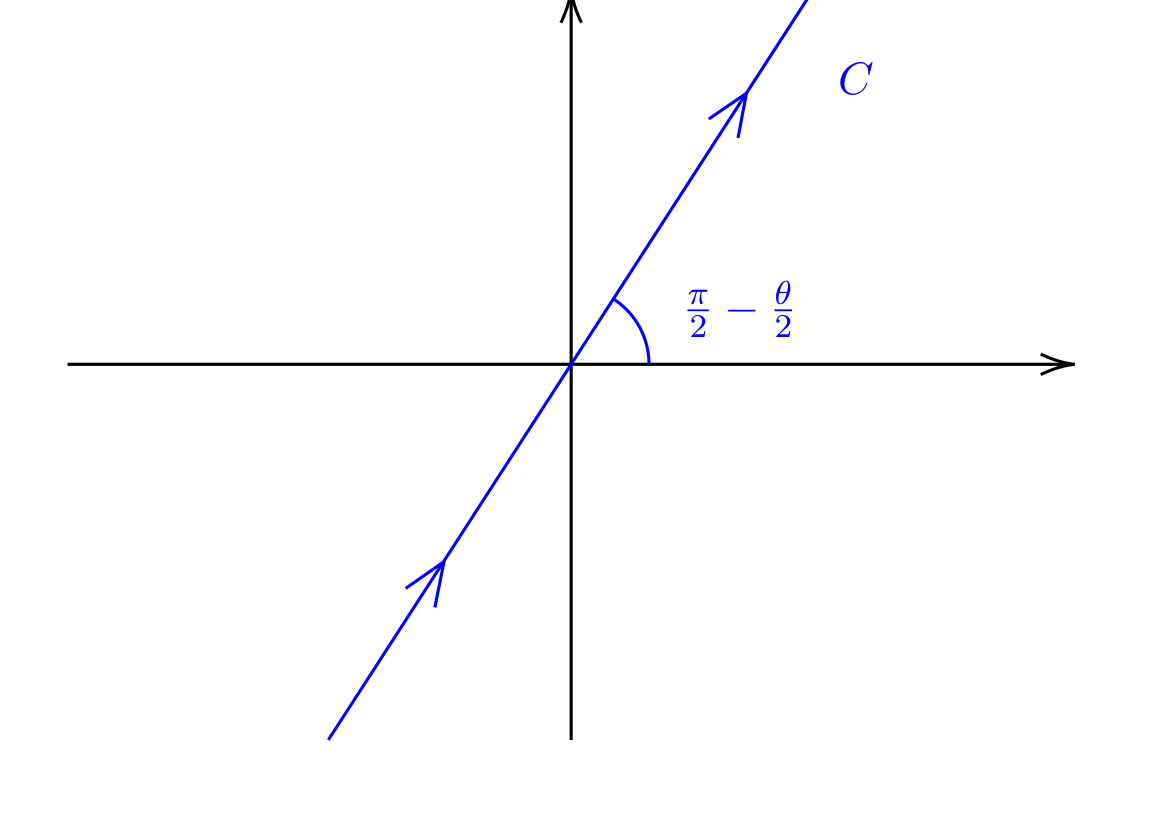
\includegraphics[width=0.42\textwidth]{figures/fig_p102_b.png}
\end{center}
% [图：原书 p.101，原图无题注]

% [原文 p.102]
一般地，设要描述积分
\[
\int_C\ee^{\lambda f(z)}
\]
经过鞍点 $z_0$ 的最速下降曲线。则 $C$ 在 $z_0$ 处的切线沿角度
\[
\frac\pi2-\frac12\operatorname{Arg}\left(f''(z_0)\right)
\]
的方向。

\begin{center}
  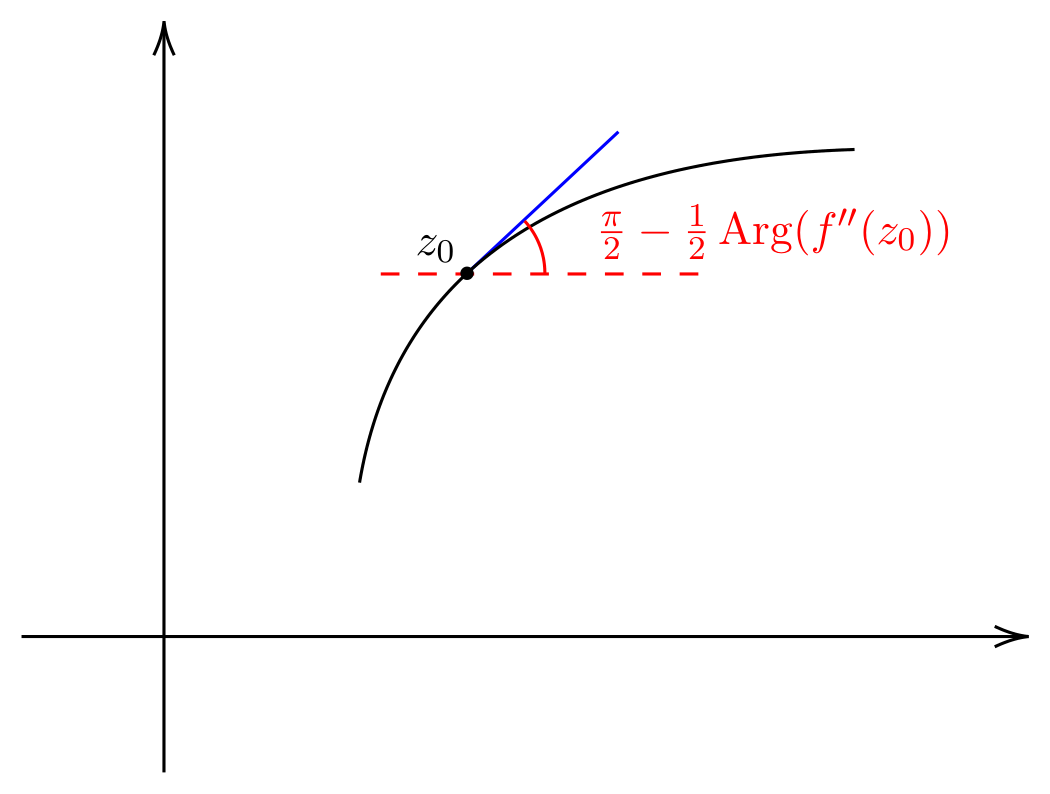
\includegraphics[width=0.42\textwidth]{figures/fig_p103_a.png}
\end{center}
% [图：原书 p.102，原图无题注]
\end{example}

\subsection{斯托克斯现象}

在渐近方法的应用中，常会遇到有多个鞍点、需要把它们全部求和的情形。然而，当我们变动模型参数时，这些渐近展开之和可能出现不连续的跳跃。这称为\emph{斯托克斯现象}（Stokes phenomenon）。这种跳跃现象其实对应重要的物理行为。我们将通过一个具体例子——\emph{艾里积分}——来解释斯托克斯现象的基本想法。

\subsection*{艾里函数}

考虑沿实轴的如下艾里积分
\[
I(\lambda):=\int_{-\infty}^{+\infty}
\ee^{\ii\lambda\left(\frac{z^3}{3}-z\right)}\rd z
=2\int_0^{+\infty}\cos\left(\lambda\left(\frac{z^3}{3}-z\right)\right)\rd z,
\]
其中 $\lambda\in\R_{>0}$。这个积分收敛，并与标准艾里函数 $\operatorname{Ai}$ 通过
\[
\operatorname{Ai}(x)=\frac1\pi\int_0^{+\infty}
\cos\left(\frac{z^3}{3}+xz\right)\rd z
\]
相联系：
\[
I(\lambda)=2\pi\lambda^{-\frac13}\operatorname{Ai}\left(-\lambda^{\frac23}\right).
\]
我们关心 $\lambda\to+\infty$ 时 $I(\lambda)$ 的渐近行为。如前面所讨论，这可以用最速下降法分析。要用这个方法，第一步是把围道 $C=\R$ 形变为最速下降围道。令
\[
f(z)=\ii\lambda\left(\frac{z^3}{3}-z\right).
\]

% [原文 p.103]
它有两个鞍点
\[
f'(z)=0\qquad\Longrightarrow\qquad z=p_\pm=\pm1.
\]
最速下降曲线是经过鞍点、并满足下列条件的围道
\begin{itemize}
  \item[①] $\operatorname{Im}f=\text{常数}$；
  \item[②] $\operatorname{Re}f\to-\infty$ 沿曲线的无穷端点。
\end{itemize}
由于
\[
f(p_\pm)=\pm\frac23\ii\lambda,
\]
就有两条分别对应鞍点 $p_\pm$ 的最速下降曲线 $C_\pm$。

为描述这些曲线，考虑流方程
\[
\frac{\rd z}{\rd u}=-\overline{f'(z)}
=\ii\lambda\left(\bar z^2-1\right),
\]
在实坐标 $z=x+\ii y$ 下它可写成
\[
\begin{cases}
\dfrac{\rd x}{\rd u}=2\lambda xy\\[2mm]
\dfrac{\rd y}{\rd u}=\lambda(x^2-y^2-1)
\end{cases}
\qquad (\lambda>0)
\]
我们可以画出相应流的方向

\begin{center}
  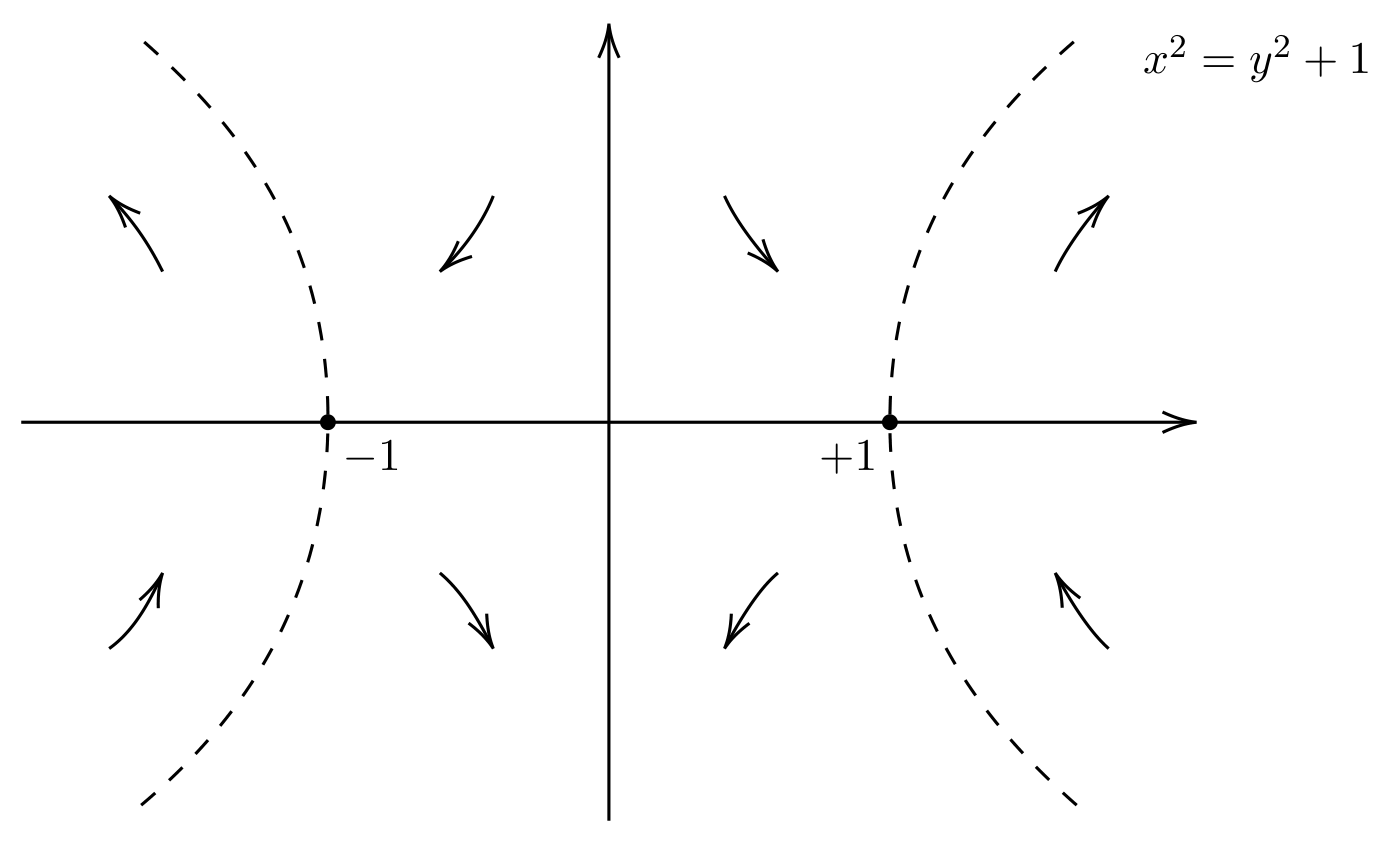
\includegraphics[width=0.60\textwidth]{figures/fig_p104_a.png}
\end{center}
% [图：原书 p.103，原图无题注]

由此可以画出曲线 $C_\pm$ 为

% [原文 p.104]
\begin{center}
  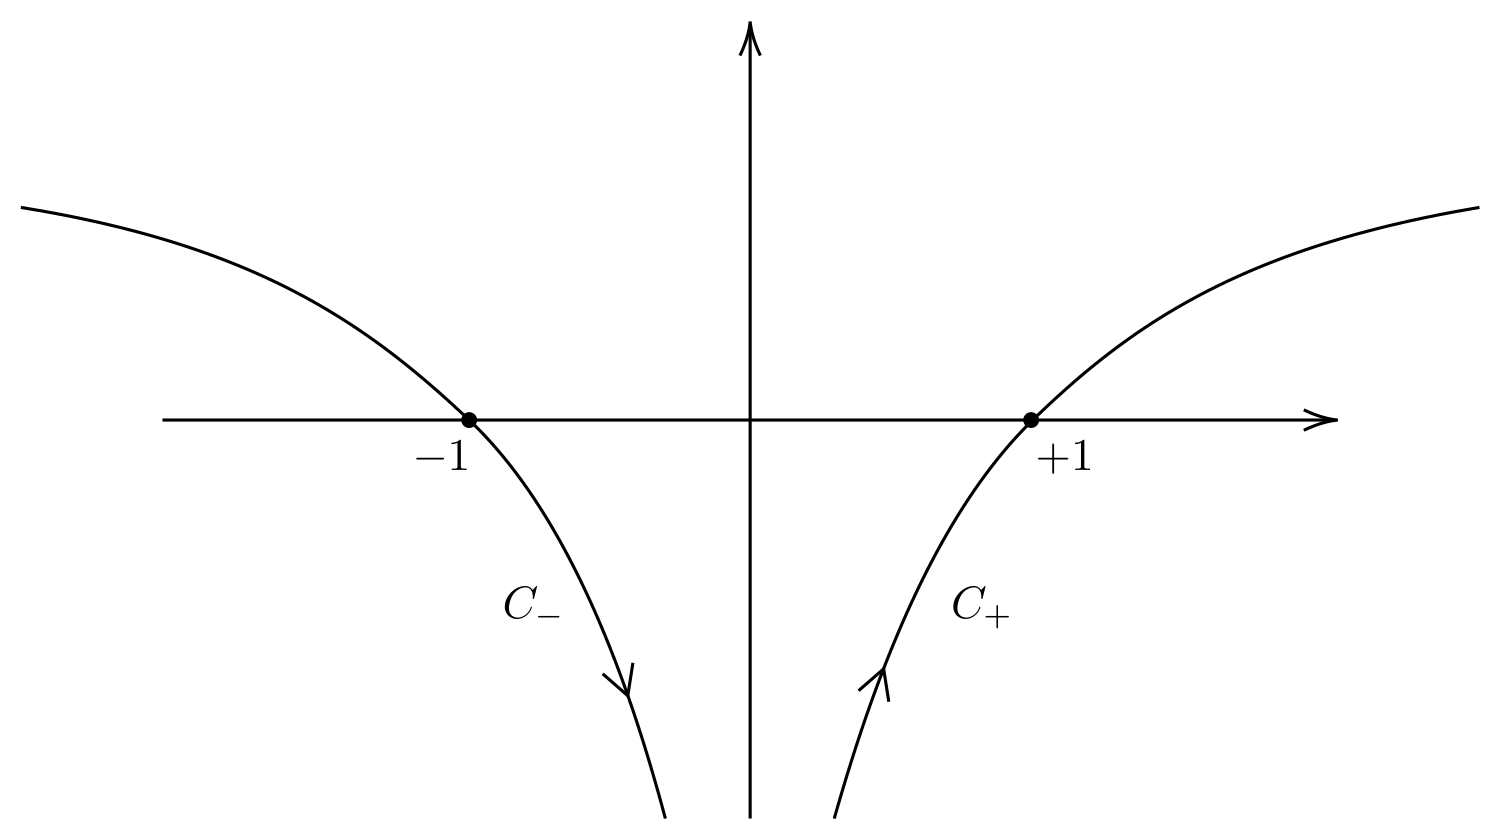
\includegraphics[width=0.62\textwidth]{figures/fig_p105_a.png}
\end{center}
% [图：原书 p.104，原图无题注]

由此可知，当 $\lambda>0$ 时
\[
I(\lambda)=\int_{\R}\ee^{\ii\lambda\left(\frac{z^3}{3}-z\right)}\rd z
=\int_{C_-}\ee^{\ii\lambda\left(\frac{z^3}{3}-z\right)}\rd z
+\int_{C_+}\ee^{\ii\lambda\left(\frac{z^3}{3}-z\right)}\rd z,
\]
即把围道 $\R$ 形变为最速下降的 $C_-+C_+$。于是由最速下降法，$I(\lambda)$ 有渐近行为
\[
I(\lambda)\simeq\sqrt{\frac{\pi}{\ii\lambda}}\,
\ee^{\frac23\ii\lambda}\left(1+O\left(\frac1\lambda\right)\right)
+\sqrt{\frac{\pi}{-\ii\lambda}}\,
\ee^{-\frac23\ii\lambda}\left(1+O\left(\frac1\lambda\right)\right),
\qquad \lambda\to+\infty.
\]

\subsection*{斯托克斯射线}

现在考虑艾里积分
\[
\int_C\ee^{\ii\lambda\left(\frac{z^3}{3}-z\right)}\rd z
\]
随 $\lambda$ 变化时的解析延拓。特别地，我们想分析
\[
\lambda\to+\infty\,\ee^{\ii\theta},
\]
即 $\lambda$ 沿 $\ee^{\ii\theta}$ 方向趋于无穷时的渐近行为。

$\lambda$ 变动时，需要相应地形变积分围道 $C$，使积分保持收敛。同样可以把 $C$ 分解为最速下降曲线 $C_\pm^\lambda$ 的组合。这些 $C_\pm^\lambda$ 与两个鞍点相联系，由下述条件刻画：
\begin{itemize}
  \item[①] $C_\pm^\lambda$ 经过鞍点 $p_\pm=\pm1$；
  \item[②] $\operatorname{Im}f$ 沿 $C_\pm^\lambda$ 为常数；
  \item[③] $\operatorname{Re}f\to-\infty$ 沿 $C_\pm^\lambda$ 的无穷端点。
\end{itemize}
其中
\[
f=\ii\lambda\left(\frac{z^3}{3}-z\right).
\]
注意
\[
\operatorname{Im}\left(f(p_\pm)\right)=\pm\frac23\operatorname{Re}\lambda.
\]
所以只要 $\operatorname{Re}\lambda\ne0$，曲线 $C_\pm^\lambda$ 就不相交，并趋向无穷时落在不同区域。

% [原文 p.105]
\begin{center}
  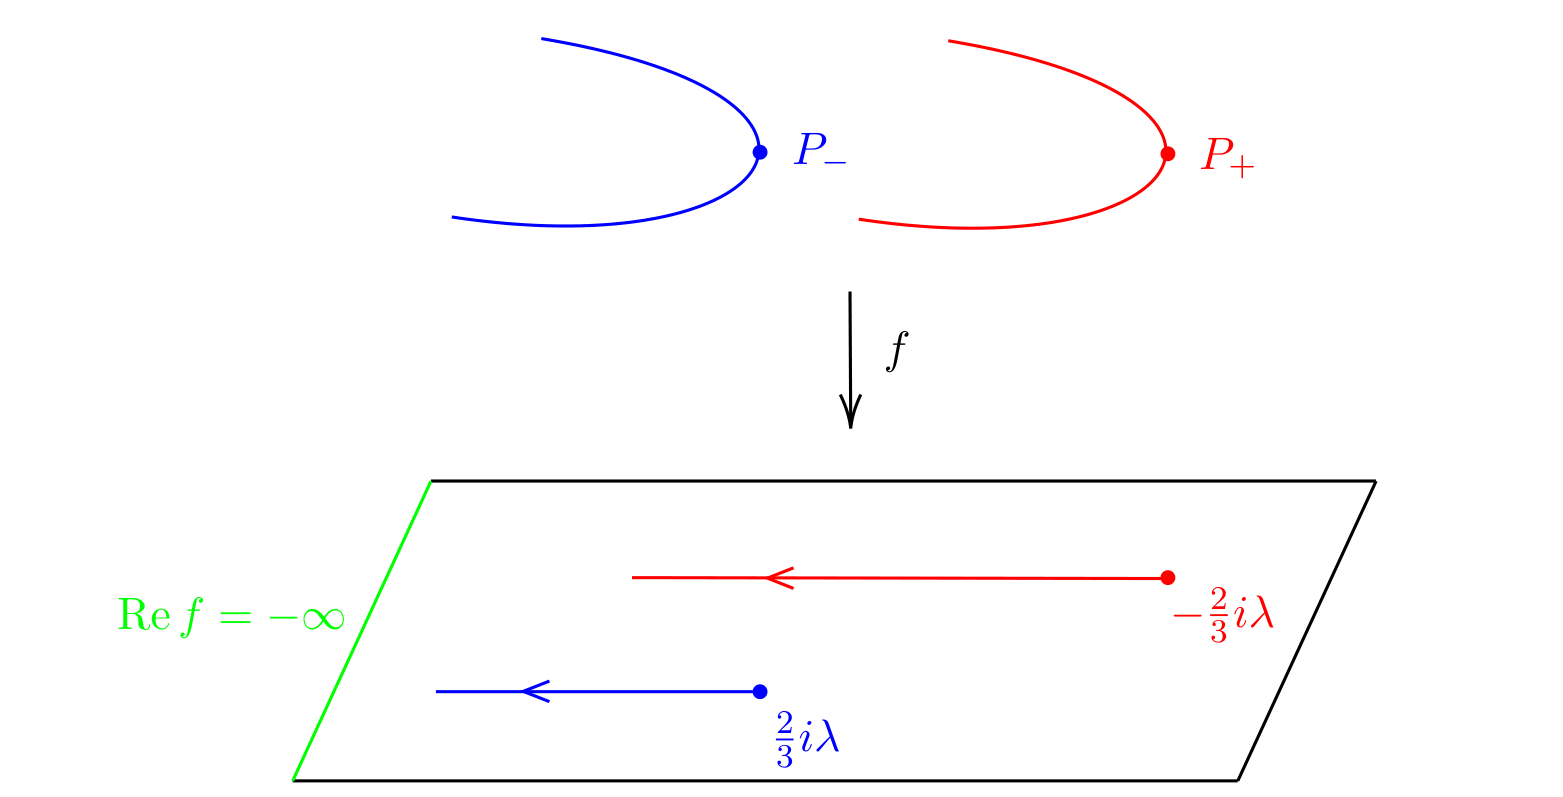
\includegraphics[width=0.68\textwidth]{figures/fig_p106_a.png}
\end{center}
% [图：原书 p.105，原图无题注]

若把围道 $C$ 形变为
\[
C=n_-C_-^\lambda+n_+C_+^\lambda,
\]
则艾里积分成为
\[
\int_C\ee^f\rd z
=n_-\int_{C_-^\lambda}\ee^f\rd z
+n_+\int_{C_+^\lambda}\ee^f\rd z.
\]
现在 $\lambda$ 变动时，圈 $C_\pm^\lambda$ 随之转动。只要 $\lambda$ 不落在轨迹 $\{\operatorname{Re}\lambda=0\}$ 上，曲线 $C_\pm^\lambda$ 就连续变化。然而当
\[
\operatorname{Re}\lambda=0,
\]
即 $\lambda$ 变成纯虚数时，
\[
\operatorname{Im}\left(f(p_-)\right)=\operatorname{Im}\left(f(p_+)\right),
\]
而
\[
\operatorname{Re}\left(f(p_\pm)\right)=\pm\frac23\operatorname{Im}\lambda.
\]
于是其中一条最速下降曲线连接两个鞍点。$\lambda$ 平面中的这两条射线
\[
\{\lambda\in\ii\R_{>0}\}\cup\{\lambda\in\ii\R_{<0}\}
\]
称为\emph{斯托克斯射线}（Stokes rays）。

% [原文 p.106]
\begin{center}
\begin{tikzpicture}[scale=0.9,>=Stealth]
  \draw[<->] (0,-1.5) -- (0,1.5);
  \node at (-1.75,0.1) {斯托克斯射线};
  \draw (2.0,-0.35) rectangle (3.5,0.35);
  \node at (2.75,0) {$\lambda$ 平面};
\end{tikzpicture}
\end{center}
% [图：原书 p.106，本图按原文重绘，图内标注已译为中文；原图无题注]

在斯托克斯射线 $\lambda\in\ii\R_{>0}$ 上：$\operatorname{Re}(f(p_+))>\operatorname{Re}(f(p_-))$。

\begin{center}
  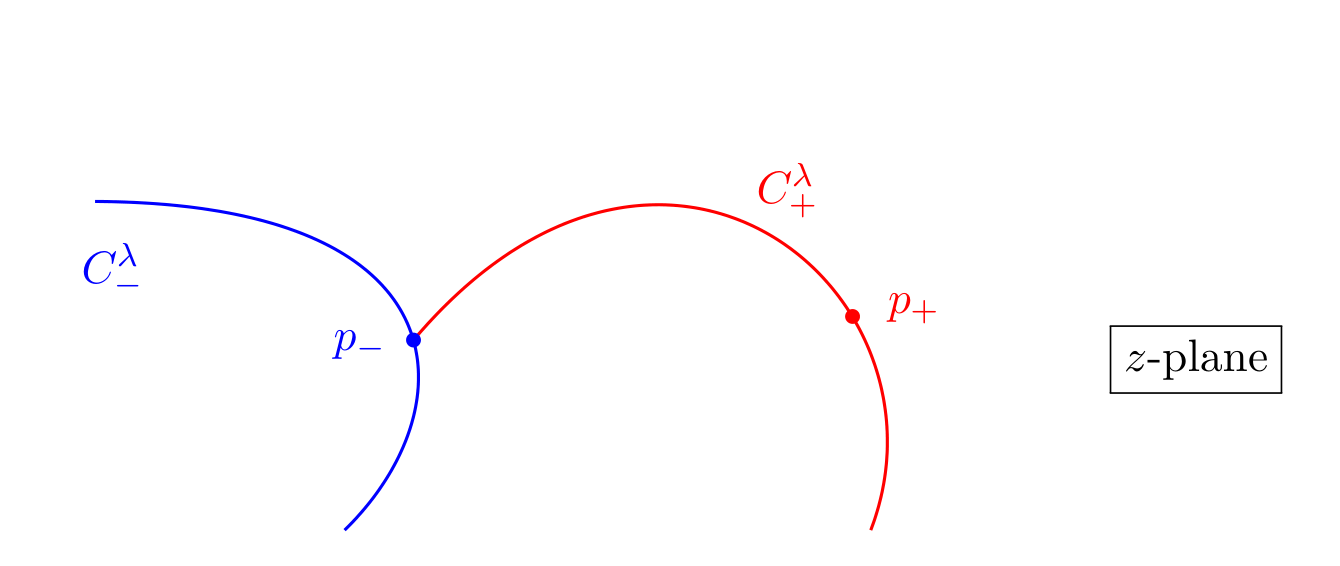
\includegraphics[width=0.62\textwidth]{figures/fig_p107_b.png}
\end{center}
% [图：原书 p.106，图内文字照原样保留]
\fignote{图内文字：$z$-plane（译：$z$ 平面）}

当我们跨过斯托克斯射线时，曲线 $C_\pm^\lambda$ 会发生离散变换。下图说明跨过其中一条斯托克斯射线的情形。

\begin{center}
  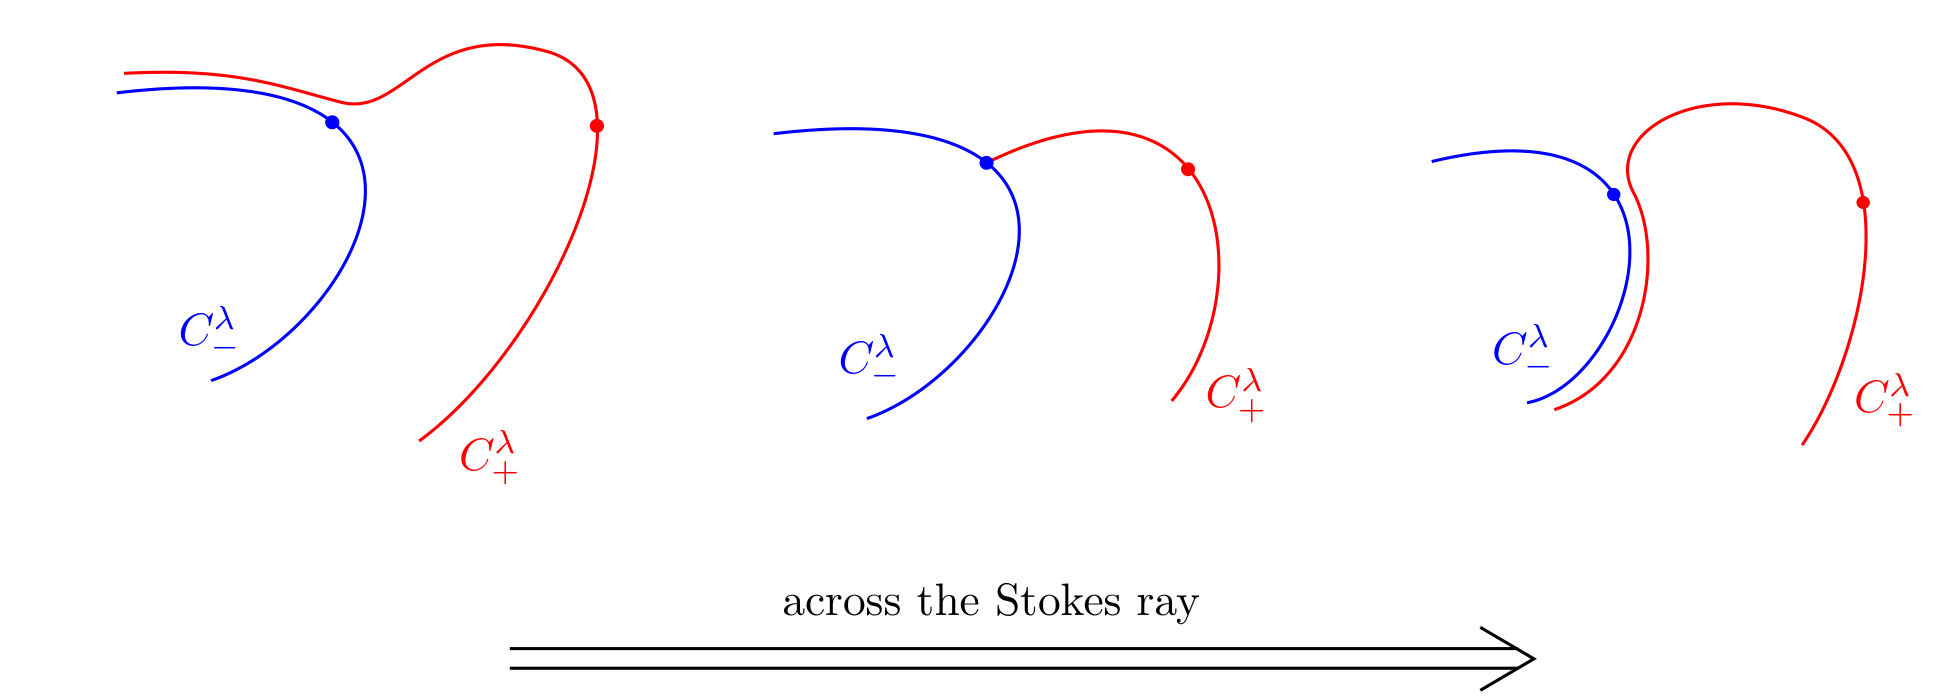
\includegraphics[width=0.75\textwidth]{figures/fig_p107_c.png}
\end{center}
% [图：原书 p.106，图内文字照原样保留]
\fignote{图内文字：across the Stokes ray（译：跨过斯托克斯射线）}

相应的围道 $C_\pm^\lambda$ 按图中所示发生变换
\[
\begin{cases}
C_-^\lambda\mapsto C_-^\lambda\\
C_+^\lambda\mapsto C_+^\lambda\pm C_-^\lambda
\end{cases}
\]
我们把上述结果用于
\[
\int_C\ee^{\ii\lambda\left(\frac{z^3}{3}-z\right)}\rd z
\]
的解析延拓：$\lambda$ 变动时相应地调整围道 $C$ 的形变。可以把围道 $C$ 分解为最速下降曲线之和
\[
C=n_-C_-^\lambda+n_+C_+^\lambda.
\]

% [原文 p.107]
于是，为使 $C$ 的形变沿解析延拓保持连续，数对 $(n_-,n_+)$ 在离开斯托克斯射线时局部为常数，但跨过斯托克斯射线时会出现跳跃
\[
\begin{cases}
n_+\mapsto n_+\\
n_-\mapsto n_-\pm n_+
\end{cases}
\]

\subsection*{渐近求和}

现在考察艾里积分的渐近行为
\[
I(\lambda)=\int_C\ee^{\ii\lambda\left(\frac{z^3}{3}-z\right)}\rd z,
\qquad \lambda\to+\infty\,\ee^{\ii\theta}.
\]
用最速下降法，先把围道 $C$ 形变为组合
\[
C=n_-C_-^\lambda+n_+C_+^\lambda.
\]
于是最速下降法给出首阶渐近行为
\[
\begin{aligned}
I(\lambda)&=n_-\int_{C_-^\lambda}\ee^{\ii\lambda\left(\frac{z^3}{3}-z\right)}\rd z
+n_+\int_{C_+^\lambda}\ee^{\ii\lambda\left(\frac{z^3}{3}-z\right)}\rd z\\
&\simeq n_-\sqrt{\frac{\pi}{\ii\lambda}}\,\ee^{\frac23\ii\lambda}
+n_+\sqrt{\frac{\pi}{-\ii\lambda}}\,\ee^{-\frac23\ii\lambda},
\qquad \lambda\to+\infty\,\ee^{\ii\theta}.
\end{aligned}
\]
注意
\begin{itemize}
  \item[①] 若 $\operatorname{Im}\lambda>0$，则 $\int_{C_+^\lambda}$ 占主导；
  \item[②] 若 $\operatorname{Im}\lambda<0$，则 $\int_{C_-^\lambda}$ 占主导。
\end{itemize}
实轴上把主导渐近行为分开的射线 $\{\operatorname{Im}\lambda=0\}$ 有时称为\emph{反斯托克斯射线}（anti-Stokes ray）。

\begin{center}
\begin{tikzpicture}[scale=0.85,>=Stealth]
  \draw (2.6,1.45) rectangle (4.1,2.15);
  \node at (3.35,1.8) {$\lambda$ 平面};
  \node at (0,0.75) {$\int_{C_+^\lambda}$ 占主导};
  \draw[<->] (-3.4,-0.3) -- (3.6,-0.3);
  \node at (1.9,-0.85) {反斯托克斯射线};
  \node at (0,-1.5) {$\int_{C_-^\lambda}$ 占主导};
\end{tikzpicture}
\end{center}
% [图：原书 p.107，本图按原文重绘，图内标注已译为中文；原图无题注]

这与前面讨论过的斯托克斯跳跃相容。例如考虑跨过斯托克斯射线 $\lambda\in\R_{>0}$ 的情形。

\begin{center}
\begin{tikzpicture}[scale=0.85,>=Stealth]
  \draw[->] (-2.6,0) -- (3.0,0);
  \draw[->] (0,-1.3) -- (0,1.7);
  \draw (2.2,1.45) rectangle (3.7,2.15);
  \node at (2.95,1.8) {$\lambda$ 平面};
  \draw[->] (-0.55,0.5) to[bend left=45] (0.6,0.55);
  \node at (-2.0,0.5) {$\int_{C_+^\lambda}$ 占主导};
\end{tikzpicture}
\end{center}
% [图：原书 p.107，本图按原文重绘，图内标注已译为中文；原图无题注]

% [本块止于原书 p.107，下接 ch02b]
% [注：§2.5 渐近方法 已在本块起头（\section{渐近方法} 在原书 p.96），其 \takeaway 留给 ch02b 在节末补写。]
